\documentclass[a4paper,12pt]{book}
\usepackage[utf8]{inputenc}
\usepackage{amsmath,amssymb,latexsym}
\usepackage{graphicx,subfigure}
\usepackage{tcolorbox}
\usepackage{wrapfig}
\usepackage{rotating}
\usepackage[margin=2.5cm]{geometry}
\newtheorem{Equation}{\indent Equation}[section]
\textwidth=6in
\renewcommand{\baselinestretch}{1.5}

\begin{document}

\author{Zachary Matheson}
\title{Everything you wish you'd known when you STARTED your PhD}
\date{Revised November 2017}

\frontmatter
\maketitle
\tableofcontents

\mainmatter
\chapter{Pairing in Nuclear Theory}

\maketitle
There are several different ways to include pairing correlations in nuclear structure calculations, many of which are based on the BCS theory of superconductors. In it, nucleon pairs can be described as quasiparticles in a nuclear superfluid. Here I will describe three different approaches for describing nuclear structure which account for pairing, each with varying degrees of generality.

\section*{BCS Theory and HF+BCS (\cite{suhonen2007nucleons,Anguiano2013})}
One way to include pairing correlations is to solve the Hartree-Fock equations and add BCS on top. This method is called HF+BCS and it does a fair job of describing nuclei near the valley of stability, but gets progressively worse the further from stability you get (see \cite{Anguiano2013}).

Basically the idea is that you use HF to take you from a system with a whole bunch of interdependent particles, which each obey a one-body Hamiltonian piece AND a two-body Hamiltonian piece, to an alternate basis in which you basically only have a one-body Hamiltonian. Then, in that basis, you solve the BCS equations on top, so you're doing BCS on a basis that doesn't exactly describe the real interaction Hamiltonian but is close enough to the real thing.

Another way of saying it is that the HF equations give you single-particle wavefunctions, in the basis which most closely approximates/diagonalizes the [two-body] Hamiltonian. So it's sort of a fictitious basis, in that your Hamiltonian is not \textit{really} diagonal, but it's as good as you're gonna get. That's what the variation does - you're varying the ground state energy according to the coefficients which give you the most ideal linear combination of starting basis functions (harmonic oscillator or whatever). But the main idea is this: that you pretend your two-body Hamiltonian is actually a one-body Hamiltonian, diagonalize it, and make the error in your approximation as small as possible.

For the next step, when you add in the BCS, you typically make (at least for even-even nuclei) the ground state ansatz $|BCS\rangle = \prod_{k>0}(u_k+v_k a_k^\dagger a_{\bar{k}}^\dagger)|0\rangle$, which doesn't conserve particle number (in fact, it's a linear superposition of pairs starting from zero pairs all the way up to $\frac{A}{2}$ pairs), but I guess it's close enough. Then you typically enforce particle number conservation some other way, perhaps by adding a Lagrange multiplier.

Next you take your pairing Hamiltonian, which I suppose would include your mean-field, now one-body Hamiltonian (which stands in for the two-body Hamiltonian you had before you performed Hartree-Fock), and you add in a new two-body potential, which this time represents the effect of pairing. Then you perform a Hartree-Fock-style calculation all over again, essentially just doing another Hartree-Fock calculation on top of your original one, except that this time you might probably have an extra Lagrange multiplier constraint in your Hamiltonian. It doesn't change anything substantial but it's good to keep in mind. There are probably other ways of constraining particle number, too, like Lipkin-Nogami, but I'm not too sure how those work.

Some other things to keep in mind:
\begin{itemize}
\item You can still think of your system in terms of the HF-basis real particle wavefunctions $a_k^\dagger |0\rangle$, with $|BCS\rangle = \prod_{k>0}(u_k+v_k a_k^\dagger a_{\bar{k}}^\dagger)|0\rangle$. Or, to simplify the math, you can invent a new "quasiparticle" such that $|BCS\rangle = \prod_{k}\alpha_k^\dagger|0\rangle$. This trick is called the Bogoliubov transformation and it looks like this:

\begin{eqnarray}
\alpha_k^\dagger = u_ka_k^\dagger-v_ka_{\bar{k}} \label{quasiparticle1}\\
\alpha_{\bar{k}}^\dagger = u_ka_{\bar{k}}^\dagger+v_ka_k \label{quasiparticle2}
\end{eqnarray}
\item A pairing gap $\Delta = 0$ seems to mean there is no energy associated with pairing. All pairs are formed below the Fermi surface, because why on Earth wouldn't they? It's free! Whereas a nonzero pairing gap means there is some energy associated with forming a pair. So the probability of forming pairs is less than one below the Fermi surface, but there's also a possibility that pairs might form outside the Fermi surface. The pairing gap basically defines how far outside the Fermi surface you can go (see p 233 of \cite{ring1980nuclear}, for ex., or p 13 of \cite{Balbuena2003}).
\item You could also do the BCS calculation using single-particle states derived from a phenomenological potential. You'd sacrifice some accuracy but gain some speed \cite{Anguiano2013}.
\end{itemize}

\section*{Hartree-Fock-Bogoliubov (HFB)  (\cite{ring1980nuclear,Balbuena2003})}
In HF theory, you find the eigenfunctions of the one-body Hamiltonian which most closely resembles the actual two-body Hamiltonian. The basic idea to HFB is that in HFB you do basically the same thing, except you can't ignore two-body interactions because of pairing. So I guess in a way you sort of find the eigenfunctions of the two-body Hamiltonian which most closely resembles the actual four-body Hamiltonian. There's a little bit more subtlety than that, because the pairing correlations mean the particles are related somehow, but that's not a bad way to envision it, because one quasiparticle has a $U$ term, which corresponds to adding a particle, and a $V$ term, which does the opposite - so it's like creating a pair all at once (see equation \ref{HFBqp})! In reality, each HFB quasiparticle is a sum of such terms, but you get the idea. In some sense, one quasiparticle $\sim$ two real particles.

By way of comparison to HF+BCS, which is a two-step process, HFB just does both steps at once to give you a single set of quasiparticle wavefunctions, instead of one set of single-particle wavefunctions based on another set of wavefunctions. The approximation in the end is better, but it is more computationally intensive than HF+BCS.

Let's see how this calculation is to be done. Suppose our Hamiltonian is:

\begin{equation}
\hat{H}=\sum\limits_{i,j} t_{ij} \hat{c}_i^\dagger \hat{c}_j + \frac{1}{4}\sum\limits_{i,j,m,n} \bar{v}_{ijmn} \hat{c}_i^\dagger \hat{c}_j^\dagger \hat{c}_n \hat{c}_m
\end{equation}

As mentioned before, let us make the following Bogoliubov transformation to make the math simpler:

\begin{equation}
\left(\begin{array}{c}
\hat{\beta} \\
\hat{\beta^\dagger}
\end{array}\right)
= \left(\begin{array}{cc}
U^\dagger & V^\dagger \\
V^\dagger & U^\dagger
\end{array}\right) \left(\begin{array}{c}
\hat{c} \\
\hat{c^\dagger}
\end{array}\right) \label{HFBqp}
\end{equation}

\noindent Now the Hamiltonian looks like this:

\begin{eqnarray}
\hat{H} = \hat{H}_0 + \sum\limits_{i,j}\hat{H}_i,j\beta_i^\dagger\beta_j + \sum\limits_{i<j}(\hat{H}_{i,j}\beta_i^\dagger\beta_j^\dagger + h.c.) + \hat{H}_{int} \nonumber\\
= \hat{H}_0 + \hat{H}_{11} + \hat{H}_{20} + \hat{H}_{40} + \hat{H}_{31} + \hat{H}_{22}
\end{eqnarray}

\noindent where $h.c.$ is the hermitian conjugate of the previous term and the term $\hat{H}_{nm}$ contains all terms with $n$ quasiparticle creation operators and $m$ annihilation operators. We'll lump the terms with 4 creation/annhilation operators into a single term $\hat{H}_{int}$, which we'll assume is small and thus ignore (sort of like the term $V(r)-\sum_{i,j}V(r_i,r_j)$ from regular Hartree-Fock theory). Let us constrain the average particle number by adding in a Lagrange multiplier term $\lambda N$. Then we vary the total energy with respect to $U$ and $V$ (which are matrices):

\begin{equation}
\delta E' = \langle\Phi_0|\hat{H}-\lambda\hat{N}|\Phi_0\rangle
\end{equation}

After that, it's really just algebra. The variation leaves some ambiguity still in the choice of $U$ and $V$, so we will choose them to make $\hat{H}_{20}=0$ and $\hat{H}_{11}$ diagonal. Additionally, the solution will look nicer if we introduce the following two densities, the traditional single-particle density from Hartree-Fock $\rho$ and a pairing tensor called $\kappa$:

\begin{eqnarray}
\rho_{ij} = \langle\Phi_0|\hat{c}_j^\dagger\hat{c}_i|\Phi_0\rangle = (VV^T)_{ij} \\
\kappa_{ij} = \langle\Phi_0|\hat{c}_j\hat{c}_i|\Phi_0\rangle = (VU^T)_{ij}
\end{eqnarray}

We can make things look \textit{even nicer} if we introduce the following notation representing the mean field $\Gamma$ and the pairing field $\Delta$:

\begin{eqnarray}
\Gamma_{kl} = \sum_{i,j} \bar{v}_{kjli}\rho_{ij} \\
\Delta_{kl} = \frac{1}{2}\sum_{i,j} \bar{v}_{klij}\kappa_{ij}
\end{eqnarray}

After we make all these substitutions, the Hamiltonian looks like:

\begin{equation}
\hat{H}-\lambda\hat{N} = \sum\limits_{i,j}\left(\left(t_{ij} + \frac{1}{2}\Gamma_{ij} - \lambda \right) \rho_{ji} + \frac{1}{2}\Delta_{ij}\kappa_{ji}^* \right) + \sum_{i}E_i \hat{\beta}_i^\dagger\hat{\beta}_i + \hat{H}_{int}
\end{equation}

\noindent where $\hat{H}_{int}$ contains all the terms with four creation/annhilation operators and $\sum_{i}E_i \hat{\beta}_i^\dagger\hat{\beta}_i$ is the diagonal form of $\hat{H}_{11}$.

Finally, putting everything back in terms of the real particle creation and annhiliation operators $c_i^\dagger$ and $c_i$ (and then dropping those in favor of their coefficients), we get the Hartree-Fock-Bogoliubov equations in their most familiar form (setting $h=\epsilon+\Gamma$):

\begin{equation}
\left(\begin{array}{cc}
h-\lambda & \Delta \\
-\Delta^* & -(h-\lambda)^*
\end{array}\right) \left(\begin{array}{c}
\hat{U_k} \\
\hat{V_k}
\end{array}\right)
= E_k\left(\begin{array}{c}
\hat{U_k} \\
\hat{V_k}
\end{array}\right)
\end{equation}

The case of rotating nuclei is interesting because experimental moments of inertia of deformed nuclei are found to be 2-3 times larger than what is calculated when pairing is ignored. Suhonen interprets this to mean that actual rotations involve the superfluid valence pairs rotating around an inert core. You can treat this by adding another constraint to $\hat{H} - \lambda\hat{N} - \omega J_x$. This is the idea behind what is called the cranking model, which describes systems in a rotating frame. It violates time-reversal just like how you've already eliminated particle number conservation. And you can add other constraints $\hat{H} - \lambda\hat{N} - \lambda_i \hat{Q}_i$ for any number of other things, like shape deformations. We use these in fission a lot.

\section*{Lipkin-Nogami}
The Lipkin-Nogami method of restoring particle number symmetry to the nucleus involves splitting the energy density into two terms:
\begin{equation*}
\mathcal{E}_{TOT} = \mathcal{E}_{HFB} + \mathcal{E}_{LN}
\end{equation*}

\noindent where $\mathcal{E}$ is computed as

\begin{equation*}
\mathcal{E}_{LN} = -\lambda_2\left(\left\langle N^2\right\rangle -N^2\right) = -2\lambda_2 \mathrm{Tr}\rho\left(1-\rho\right)
\end{equation*}

$\lambda_2$ is evaluated on every iteration using the updated densities form the previous iteration, starting from some initial value you can set in the input. It is also possible in HFODD to fix the value of lambda and not update it for each new iteration, if you're into that kind of thing. It is given approximately via the seniority-pairing interaction by

\begin{equation*}
\lambda_2 = \frac{G}{4}\frac{\mathrm{Tr}(1-\rho)\kappa \mathrm{Tr}\rho\kappa-2\mathrm{Tr}(1-\rho)^2\rho^2}{\left[\mathrm{Tr}\rho(1-\rho)\right]^2-2\mathrm{Tr}\rho^2(1-\rho)^2}
\end{equation*}

\noindent where

\begin{equation*}
G = G_{eff} = -\frac{\bar{\Delta}^2}{E_{pair}}, \qquad E_{pair} = -\frac{1}{2}\mathrm{Tr}\Delta\kappa, \qquad \bar{\Delta} = \frac{\mathrm{Tr}\Delta\rho}{\mathrm{Tr}\rho}
\end{equation*}

The UNEDF functionals included pairing strengths for both protons and neutrons as part of the Skyrme parameter set when they were optimizing, so the pairing strength is actually given as a parameter instead of computed from the densities in (for example) HFODD $\leftarrow$ Double-check this! But I think that's how it'll work? I'm getting lost in the source trying to find out... (4-19-2017)

\section*{Just a note...}
...and I'm not sure where exactly to put this, but here goes: I like the idea of recasting nuclear structure, and especially applications with heavy nuclei such as fission, in terms of a DFT framework, because in principle a DFT framework is (or can be) exact as a way of taking into account all the quantum properties of the underlying nuclear degrees of freedom. And if you're clever about it, you can use ab initio approaches to inform or develop new and useful EDFs. But I don't know what would be the best way to do that. If you just fit a Skyrme funcitonal to some quantities calculated by an ab initio method, you really aren't doing anything better than just fitting it to experimental quantities - in fact, the experimental quantities should in principle be better! So there's a non-trivial issue to solve. It seems like something that should be doable - use an ab initio method to derive a new type of EDF with perhaps a new and better parameterization, but right now that bridge feels like a missing link. There might be some hints, though, in the references found in section 2.3 of \cite{Schunck2015error_analysis}

%\bibliography{writeup} % Pairing
\chapter{Time-dependent Hartree-Fock and the inertia tensor}

Originally this development is based on \cite{Engel1975}, and a retelling in notes by Nicolas which I have on paper but not digitally.


Some of this (specifically that relating to the inertia tensor and the cranking approximation) is mentioned in \cite{Baran2011}


The HFB matrix looks different depending on your basis (obviously...). In the single-particle basis, it has the form

\begin{equation}
\mathcal{H} = \left(\begin{array}{cc}
h & \Delta \\ 
-\Delta* & -h^*
\end{array} \right)
\end{equation}

\noindent with an associated density

\begin{equation}
\mathcal{R} = \left(\begin{array}{cc}
\rho & \kappa \\ 
-\kappa^* & 1-\rho^*
\end{array} \right)
\end{equation}

\noindent Or something like that. I might have the signs and stars wrong.

In the quasiparticle basis, on the other hand, these matrices look like this:

\begin{equation}
\mathcal{H} = \left(\begin{array}{cc}
E & 0 \\ 
0 & -E
\end{array} \right),      
\mathcal{R} = \left(\begin{array}{cc}
0 & 0 \\ 
0 & 1
\end{array} \right)
\end{equation}

\noindent At finite temperatures $T>0$, the density is slightly modified:

\begin{equation}
\mathcal{R} = \left(\begin{array}{cc}
f & 0 \\ 
0 & 1-f
\end{array} \right)
\end{equation}

What is done in ATDHFB (and, so far as I can tell, also in QRPA) is to expand your density $\mathcal{R}$ around some $\mathcal{R}_0$, which in QRPA corresponds to the HFB ground state density (I think) and in ATDHFB $\mathit{can}$ be the HFB ground state density (in practice, I think that is indeed what's most often done). The expansion parameter $\chi(t)$ works out to be, in some sense, a canonical coordinate or momentum or something like unto it. For small perturbations around the minumum, the system looks like a harmonic oscillator in time, described by the ATDHFB equations $i\dot{\mathcal{R}} = \left[\mathcal{H, R}\right]$. In ATDHFB, you find that the most common perturbations are collective coordinate changes (corresponding to shape deformations). Writing your derivatives in terms of these collective variables

\begin{equation}
\frac{d\mathcal{R}}{dt} = \frac{d\mathcal{R}}{dq}\frac{dq}{dt}
\end{equation}

\noindent and then writing everything in terms of $\chi(t)$ and $\dot{\chi}(t)$, you find an expression for the energy which looks like a kinetic energy, with $\dot{q}$'s or $\dot{\chi}$'s as your "velocity."

Begin by expanding $\mathcal{R}\approx\mathcal{R}_0+\mathcal{R}_1$ and, correspondingly, $\mathcal{H}\approx\mathcal{H}_0+\mathcal{H}_1$. $\mathcal{R}_0$ and $\mathcal{H}_0$ are both diagonal in the quasiparticle basis, so it makes sense to start from there. Expand your commutator $i\dot{\mathcal{R}} = \left[\mathcal{H, R}\right]$ in terms of these guys where possible, and a lot of this stuff will turn out to be pretty trivial. The difficult part will be expressing $\mathcal{H}_1$ in the quasiparticle basis. For that, you'll probably need to start with $\mathcal{R}$ and $\mathcal{H}$ in the single-particle basis

\begin{equation}
\mathcal{R} = \left(\begin{array}{cc}
\rho & \kappa \\ 
-\kappa^* & 1-\rho^*
\end{array} \right)
\approx
\left(\begin{array}{cc}
\rho_0 & \kappa_0 \\ 
-\kappa^*_0 & 1-\rho^*_0
\end{array} \right) + 
\left(\begin{array}{cc}
\rho_1 & \kappa_1 \\ 
-\kappa^*_1 & -\rho^*_1
\end{array} \right)
\end{equation}

\noindent Then you'll construct $\mathcal{H}$ in this basis by explicitly evaluating $h_{ij} = t_{ij} + \sum_{mn}\bar{v}_{imjn}\rho_{nm}$ and $\Delta_{ij} = \frac{1}{2}\sum_{mn}\bar{v}_{ijmn}\kappa_{mn}$ (double-check the indices and expressions before use, of course!). You can transform this into the quasiparticle basis, or the other part into the single particle basis (or in reality, I think you'll have to do a bit of both), and that'll give you the full expression. However, in the cranking approximation, we actually apparently ignore this whole second term because we assume that small changes in the density will not affect the mean field ($\mathcal{R}\approx\mathcal{R}_0 \Rightarrow\mathcal{H}_1\approx0$)

To close out this chapter, a good soul-searching question you should ask yourself someday (just to make sure you understand what's going on) is, if you take away the ATDHFB or GCM or and other model-dependence, what is still left? What is the essence of the inertia tensor, and what do you risk leaving behind in each of these models? Because the inertia tensor exists even in older models, too. Clearly, there's something that people associate with a collective inertia that dates back many years. % TDHF, inertia
\chapter{RPA vs ATDHF and QRPA vs ATDHFB}

I suspect the "Random Phase" in RPA refers to the $\chi$ which pops up when we rewrite the density $\rho$ about the HF/HFB ground state density $\rho_0$ in the following way:

\begin{equation}
\rho = e^{i\chi} \rho_0 e^{-i\chi}
\end{equation}

\noindent The "Approximation" part of RPA is when we expand $\rho$ for small perturbations about the ground state, truncating the series at (typically) first- or second-order in $\chi$.

In static RPA, once we've expanded the density and the energy out to second-order in $\chi$, you can rewrite the second-order energy term as a vector-matrix-vector multiplication:

\begin{equation}
E^{(2)} = \frac{1}{2}\left(\chi^\dagger, -\chi^T\right) \left(\begin{array}{cc}
A & B \\
B^* & A^*
\end{array}\right) \left(\begin{array}{c}
\chi \\
-\chi^*
\end{array}\right)
\end{equation}

\noindent This matrix is what is called the RPA matrix (or sometimes the stability matrix, since $|E^{(2)}|>0$ corresponds to $\rho_0$ being a minimum, I think).

This matrix actually pops up again when you start from the TDHF equations $i\hbar\frac{\partial\rho}{\partial t} = [h, \rho]$. Expand the density around its ground state in terms of some parameter $\chi$ again, except this time, $\chi$ is time-dependent. If you work in the HF basis where the density and the energy are both diagonal, and keeping terms to first order this time, you eventually arrive at

\begin{equation}
i\hbar(n_j-n_i)\frac{\partial}{\partial t}\left(\begin{array}{c}
\chi_{ij} \\
\chi_{ij}^*
\end{array}\right) = \left(\begin{array}{cc}
A_{ij\mu\nu} & B_{ij\mu\nu} \\
B^*_{ij\mu\nu} & A^*_{ij\mu\nu}
\end{array}\right) \left(\begin{array}{c}
\chi_{\mu\nu} \\
-\chi^*_{\mu\nu}
\end{array}\right)
\end{equation}

So apparently this matrix is significant somehow. % RPA vs. ATDHF
\chapter{Temperature-dependent ATDHFB}

A lot of these ideas I'm getting from \cite{Schunck2015FTfission} as well as Nicolas' own temperature-dependent HFB notes.

\section{A brief overview of the theory}

As in any statistical theory, one first must determine which sort of ensemble properly describes the system. Nuclei have (in principle) conserved number of particles; however in HFB theory, that's somewhat flexible since the BCS transformation explicitly breaks particle number symmetry. In principle we should perhaps use a microcanonical ensemble to describe a nucleus as a closed, isolated system, but that turns out to be challenging to solve because it requires a full knowledge of the eigenspectrum of the nucleus. Using that quirk of HFB theory, we wiggle our way out of this hairiness\footnote{You can wave your hands here and say that finite temperatures let you break superfluid pairs, and so the number of ``quasiparticles" (which you could argue might have referred to pairs before but now might also include individual particles) can change.} to instead describe our system using the grand canonical ensemble, and this turns out to be tractable.

Moving forward by minimizing the grand potential $\Omega$ gives us for the density:
\begin{equation*}
\hat{D} = \frac{1}{Z}e^{-\beta\left(\hat{H}-\mu\hat{N}\right)}
\end{equation*}

\noindent with associated partition function

\begin{equation*}
Z = Tr\left[e^{-\beta\left(\hat{H}-\mu\hat{N}\right)}\right]
\end{equation*}

Getting specifically to our particular choice of mean-field Hamiltonian, we substitute in some one-body operator for the exponent:

\begin{equation*}
\hat{D}_{HF} = \frac{1}{Z}e^{-\beta\hat{K}}, Z = Tr\left[e^{-\beta\hat{K}}\right]
\end{equation*}

\noindent where in the plain ol' Hartree Fock case, $\hat{K} = \sum_{ij}K_{ij}c_i^\dagger c_j$ (in the HFB case, $\hat{K}$ is a sum of all different one-body operator types, but it's the same basic idea).

Defining the HF density matrix $\rho_{ij}=Tr\left[\hat{D}_{HF}c_j^\dagger c_i\right]$, we can show the following useful correspondence relations:

\begin{align*}
\rho &= \frac{1}{1+e^{\beta\hat{K}}} \\
Tr\left[\hat{D}_{HF}\hat{A}\right] &= tr\left[\rho\hat{A}\right] = \sum_{ij}\rho_{ij}\hat{A}_{ij}
\end{align*}

\noindent where $\hat{A}$ is some operator in the single-particle basis. Similar things happen for the HFB case. At the end of the day in HFB, things work out to be pretty similar to the way they were before, except the density in the quasiparticle basis is replaced by

\begin{equation*}
\mathcal{R} =
\left(\begin{array}{cc}
0 & 0 \\
0 & 1
\end{array}\right)
\rightarrow
\left(\begin{array}{cc}
f & 0 \\
0 & 1-f
\end{array}\right)
\end{equation*}

\noindent Obviously there's a lot more richness to it than that, but this helps to at least see the basic skeleton of what changes at finite temperature.

\section{Temperature-Dependent ATDHFB}

Let us quickly review the essence of Time-Dependent Hartree-Fock-Bogoliubov (TDHFB). The fundamental assumption of TDHFB is that a system which is a Slater determinant at time $t=0$ and which is then allowed to evolve in time will remain a Slater determinant at all times $t$. This assumption allows us to write to TDHFB equation:

\begin{equation*}
i\hbar \mathcal{\dot{R}} = \left[\mathcal{H},\mathcal{R}\right]
\end{equation*}

\noindent where in the single-particle basis

\begin{equation*}
\mathcal{\tilde{H}} = 
\left(\begin{array}{cc}
h-\lambda & \Delta \\
-\Delta^* & -h^*+\lambda
\end{array}\right), 
\qquad \mathcal{\tilde{R}} = 
\left(\begin{array}{cc}
\rho & \kappa \\
-\kappa^* & 1-\rho^*
\end{array}\right)
\end{equation*}

The \textit{additional} assumption that collective motion is slow compared to single particle motion of the system is called the \textit{adiabtic approximation}, and the consequent model is called Adiabatic Time-Dependent Hartree-Fock-Bogoliubov (ATDHFB). Historically, the reason for this assumption comes from microscopic-macroscopic models of nuclear fission, where the dynamics of the system are described by a few collective shape variables and their derivatives (you might think of them semiclassically as coordinates and velocities). The adiabatic approximation is implicit in this assumption. ATDHFB provides the bridge for bringing this useful framework into a self-consistent, fully-microscopic picture.

Once the system is described in terms of collective coordinates and velocities, the energy can be expressed as the sum of a ``potential" term (which depends on the coordinates) and a ``kinetic" term (which depends on the velocities). Our goal is to understand the kinetic part of the energy, which in some sense describes the dynamics of, for example, a fissioning nucleus, in terms of the first few multipole moments of the nucleus. A key component of this will be the inertia tensor $\mathcal{M}$, which plays the role of the ``mass": $E_{kin}\sim\frac{1}{2}\mathcal{M}\dot{q}^2$

\subsection{Review of ATDHFB}

With the adiabatic assumption in place, we can write the density as an expansion around some time-even zeroth-order density:

\begin{align*}
\mathcal{R}(t) 
&= e^{i\chi(t)}\mathcal{R}_0(t)e^{-i\chi(t)} \\
&= \mathcal{R}_0 + \mathcal{R}_1 + \mathcal{R}_2 + \dots
\end{align*}

\noindent where $\chi$ is assumed to be ``small" (which is explained more rigorously in \cite{Baranger1978}) and

\begin{align}\label{eqn:densities}
\mathcal{R}_1 &= i\left[\chi, \mathcal{R}_0\right] \\
\mathcal{R}_2 &= \frac{1}{2}\left[\left[\chi, \mathcal{R}_0\right], \chi\right] 
\end{align}

\noindent The HFB matrix, being a function of $\mathcal{R}$, is likewise expanded:

\begin{equation*}
\mathcal{H} = \mathcal{H}_0 + \mathcal{H}_1 + \mathcal{H}_2 + \dots
\end{equation*}

\noindent and together $\mathcal{R}$ and $\mathcal{H}$ are plugged into the TDHFB equation. Gathering terms in powers of $\chi$:

\begin{align}\label{eqn:ATDHFB_eqns}
i\hbar\mathcal{\dot{R}}_0 &= \left[\mathcal{H}_0, \mathcal{R}_1\right] + \left[\mathcal{H}_1, \mathcal{R}_0\right] \\
i\hbar\mathcal{\dot{R}}_1 &= \left[\mathcal{H}_0, \mathcal{R}_0\right] + \left[\mathcal{H}_0, \mathcal{R}_2\right]
 + \left[\mathcal{H}_1, \mathcal{R}_1\right] + \left[\mathcal{H}_2, \mathcal{R}_0\right]
\end{align}

\noindent These two equations are the ATDHFB equations. They can be solved self-consistently to find both $\chi$ and $\mathcal{R}_0$; however, this is rarely done in practice. More commonly what is done is to exploit the fact that solutions to the ATDHFB equations are (by design) \textit{close} to true HFB solutions. We then take HFB solutions and compute their time derivatives by the first ATDHFB equation to get ATDHFB-like behavior without going through the full trouble of ATDHFB.

One nice feature of using true HFB solutions instead of ATDHFB solutions is that the matrix $\mathcal{H}_0$ is diagonal in the HFB basis.

Finally, the total energy of the system is found to be

\begin{equation*}
E(\mathcal{R}) = E_{HFB} + \frac{1}{2}\mathrm{Tr}\left(\mathcal{H}_0\mathcal{R}_1\right) + \frac{1}{2}\mathrm{Tr}\left(\mathcal{H}_0\mathcal{R}_2\right) + \frac{1}{4}\mathrm{Tr}\left(\mathcal{H}_1\mathcal{R}_1\right)
\end{equation*}

\noindent The ``kinetic energy" of the system is given by the latter two terms, which (as I'll show explicitly in a moment), are both second order in $\chi$.

\subsection{Relation between $\chi$ and $\dot{\mathcal{R}}$}\label{sect:chi-rdot}

Eventually we'll want to express the energy in terms of the multipole moments $q$ and their derivatives, but for now we will content ourselves with expressing the energy in terms of $\mathcal{R}$ and $\dot{\mathcal{R}}$. From the first ATDHFB equation:

\begin{equation*}
i\hbar\mathcal{\dot{R}}_0 = \left[\mathcal{H}_0, \mathcal{R}_1\right] + \left[\mathcal{H}_1, \mathcal{R}_0\right]
\end{equation*}

Working in the HFB quasiparticle basis, we have (at finite temperatures)

\begin{equation*}
\mathcal{H}_0 = 
\left(\begin{array}{cc}
E & 0 \\
0 & -E
\end{array}\right), 
\qquad \mathcal{R}_0 = 
\left(\begin{array}{cc}
f & 0 \\
0 & 1-f
\end{array}\right)
\end{equation*}

\noindent Note that the block matrices $E$ and $f$ are both diagonal. In this same basis, we can also divide the perturbation matrix $\chi$ and the first-order energy $\mathcal{H}_1$ in the same block matrix form:

\begin{equation*}
\qquad \chi = 
\left(\begin{array}{cc}
\chi^{11} & \chi^{12} \\
\chi^{21} & \chi^{22}
\end{array}\right),
\qquad \mathcal{H}_1 = 
\left(\begin{array}{cc}
\mathcal{H}_1^{11} & \mathcal{H}_1^{12} \\
\mathcal{H}_1^{21} & \mathcal{H}_1^{22}
\end{array}\right)
\end{equation*}

\noindent Ultimately, by using the equations \ref{eqn:densities}, we arrive at the result:

\begin{align}\label{eqn:chi-rdot_uncranked}
\begin{aligned}
\hbar \dot{\mathcal{R}}_{(0),ab}^{11} &= (E_a-E_b)(f_b-f_a)\chi_{ab}^{11} + (f_b-f_a)\mathcal{H}^{11}_{(1),ab} \\
\hbar \dot{\mathcal{R}}_{(0),ab}^{12} &= (E_a+E_b)\left(1-(f_a+f_b)\right)\chi_{ab}^{12} + \left(1-(f_a+f_b)\right)\mathcal{H}^{12}_{(1),ab} \\
\hbar \dot{\mathcal{R}}_{(0),ab}^{21} &= (E_a+E_b)\left(1-(f_a+f_b)\right)\chi_{ab}^{21} - \left(1-(f_a+f_b)\right)\mathcal{H}^{21}_{(1),ab} \\
\hbar \dot{\mathcal{R}}_{(0),ab}^{22} &= (E_a-E_b)(f_b-f_a)\chi_{ab}^{22} - (f_b-f_a)\mathcal{H}^{22}_{(1),ab}
\end{aligned}
\end{align}

It is common (the so-called ``cranking approximation") to assume that changes in the density have approximately no effect on the mean field, in which case these relations reduce to

\begin{tcolorbox}
\begin{align}\label{eqn:chi-rdot}
\begin{aligned}
\hbar \dot{\mathcal{R}}_{(0),ab}^{11} &= (E_a-E_b)(f_b-f_a)\chi_{ab}^{11} \\
\hbar \dot{\mathcal{R}}_{(0),ab}^{12} &= (E_a+E_b)\left(1-(f_a+f_b)\right)\chi_{ab}^{12} \\
\hbar \dot{\mathcal{R}}_{(0),ab}^{21} &= (E_a+E_b)\left(1-(f_a+f_b)\right)\chi_{ab}^{21} \\
\hbar \dot{\mathcal{R}}_{(0),ab}^{22} &= (E_a-E_b)(f_b-f_a)\chi_{ab}^{22}
\end{aligned}
\end{align}
\end{tcolorbox}

\noindent\textit{Sanity Check:} In the $T=f=0$ case, the $^{11}$ and $^{22}$ terms vanish completely and we are left with the familiar [zero-temperature] ATDHFB equations:

\begin{align*}
\hbar \dot{\mathcal{R}}_{(0),ab}^{12} &= (E_a+E_b)\chi_{ab}^{12} + \mathcal{H}^{12}_{(1),ab} \\
\hbar \dot{\mathcal{R}}_{(0),ab}^{21} &= (E_a+E_b)\chi_{ab}^{21} - \mathcal{H}^{21}_{(1),ab}
\end{align*}

Another thing we must be careful of is the case of degenerate states. In such an event, $E_a=E_b$ and $f_a=f_b$, leading again to $\mathcal{\dot{R}}^{11}_{(0),ab}=\mathcal{\dot{R}}^{22}_{(0),ab}=0$ (but I emphasize that this is only for this particular pair of states $|a\rangle$ and $|b\rangle$).

A third, rather pedantic case to be aware of is the example of a two-state system. In that case, $f_a+f_b=1$ and then the opposite happens; namely, $\mathcal{\dot{R}}^{12}_{(0),ab}=\mathcal{\dot{R}}^{21}_{(0),ab}=0$ while $\mathcal{\dot{R}}^{11}_{(0),ab}\neq0, \mathcal{\dot{R}}^{22}_{(0),ab}\neq0$

\subsection{Kinetic Energy at Finite Temperature}

As mentioned previously, the expression for the ``kinetic" energy of the system is given by:

\begin{equation*}
E_{kin}(\mathcal{R}) = \frac{1}{2}\mathrm{Tr}\left(\mathcal{H}_0\mathcal{R}_2\right) + \frac{1}{4}\mathrm{Tr}\left(\mathcal{H}_1\mathcal{R}_1\right)
\end{equation*}

\subsubsection{Term proportional to $\mathcal{R}_2$}

It can be shown that

\begin{equation*}
\mathrm{Tr}\left(\mathcal{H}_0\mathcal{R}_2\right) = \frac{1}{2}\mathrm{Tr}\left(\left[\chi,\mathcal{H}_0\right]\left[\chi,\mathcal{R}_0\right]\right)
\end{equation*}

\noindent which leads to

\begin{equation*}
\left[\chi, \mathcal{H}_0\right] = \left(\begin{array}{cc}
[\chi^{11},E] & -\left\{\chi^{12},E\right\} \\
\left\{\chi^{21},E\right\} & -[\chi^{22},E]
\end{array}\right), \qquad
\left[\chi, \mathcal{R}_0\right] = \left(\begin{array}{cc}
[\chi^{11},f] & \chi^{12}-\left\{\chi^{12},f\right\} \\
-\chi^{21}+\left\{\chi^{21},f\right\} & -[\chi^{22},f]
\end{array}\right)
\end{equation*}

\begin{align}\label{eqn:H0R2}
\begin{aligned}
\mathrm{Tr}\left(\mathcal{H}_0\mathcal{R}_2\right) = \frac{1}{2}
&\mathrm{Tr} \left([\chi^{11},E][\chi^{11},f] + \left\{\chi^{12},E\right\}(\chi^{21}-\{\chi^{21},f\})\right. \\
&\left.+ \left\{\chi^{21},E\right\}(\chi^{12}-\{\chi^{12},f\}) + [\chi^{22},E][\chi^{22},f]\right)
\end{aligned}
\end{align}

Since $E$ and $f$ are diagonal, we can simplify expressions involving commutators and anticommutators. If $A$ is an arbitrary matrix and $D$ is diagonal, then

\begin{align*}
[A,D]_{\mu\nu} &= (D_\nu-D_\mu)A_{\mu\nu} \\
\left\{A,D\right\}_{\mu\nu} &= (D_\mu+D_\nu)A_{\mu\nu} \\
A_{\mu\nu}-\left\{A,D\right\}_{\mu\nu} &= (1-D_\mu-D_\nu)A_{\mu\nu}
\end{align*}

\noindent Then this energy term becomes

\begin{align*}
\frac{1}{2}\mathrm{Tr}\left(\mathcal{H}_0\mathcal{R}_2\right) = \frac{1}{4}
& \left[(E_b-E_a)(f_a-f_b)\chi^{11}_{ab}\chi^{11}_{ba} + (E_a+E_b)(1-f_a-f_b)\chi^{12}_{ab}\chi^{21}_{ba}\right. \\
&\left.+ (E_a+E_b)(1-f_a-f_b)\chi^{21}_{ab}\chi^{12}_{ba} + (E_b-E_a)(f_a-f_b)\chi^{22}_{ab}\chi^{22}_{ba}\right]
\end{align*}

\noindent If you wanted to get \textit{really} crazy (and we'll see in a bit why this might actually be okay), you could even throw in some extra delta functions to get this:

\begin{align*}
\frac{1}{2}\mathrm{Tr}\left(\mathcal{H}_0\mathcal{R}_2\right) = \frac{1}{4}
& \left[(E_b-E_a)(f_a-f_b)\delta_{a\alpha}\delta_{b\beta}\chi^{11}_{\alpha\beta}\chi^{11}_{ba} + (E_a+E_b)(1-f_a-f_b)\delta_{a\alpha}\delta_{b\beta}\chi^{12}_{\alpha\beta}\chi^{21}_{ba}\right. \\
&\left.+ (E_a+E_b)(1-f_a-f_b)\delta_{a\alpha}\delta_{b\beta}\chi^{21}_{\alpha\beta}\chi^{12}_{ba} + (E_b-E_a)(f_a-f_b)\delta_{a\alpha}\delta_{b\beta}\chi^{22}_{\alpha\beta}\chi^{22}_{ba}\right]
\end{align*}

\noindent Note that this now has the general form

\begin{tcolorbox}
\begin{align}\label{eqn:H0R2_inertia}
\frac{1}{2}\mathrm{Tr}\left(\mathcal{H}_0\mathcal{R}_2\right) = &
 \mathcal{\bar{M'}}^{11,11}_{\alpha\beta ab}\chi^{11}_{\alpha\beta}\chi^{11}_{ba} +
 \mathcal{\bar{M'}}^{12,21}_{\alpha\beta ab}\chi^{12}_{\alpha\beta}\chi^{21}_{ba} +
 \mathcal{\bar{M'}}^{21,12}_{\alpha\beta ab}\chi^{21}_{\alpha\beta}\chi^{12}_{ba} +
 \mathcal{\bar{M'}}^{22,22}_{\alpha\beta ab}\chi^{22}_{\alpha\beta}\chi^{22}_{ba}
\end{align}
\end{tcolorbox}

\noindent where everything that isn't a $\chi$ has just been kind of absorbed into a single coefficient.

Let's pause here for just a second and think about what we just did. Remember that our goal all along has been to treat this piece of the energy as sort of a ``kinetic energy term" describing motion in a space of collective shape deformation coordinates. Then just now we found that, sure enough, we can factor this particular chunk into something that looks \textit{kind of} like $\frac{1}{2}mv^2$. And we already know from \ref{eqn:chi-rdot} that $\chi$ is related to $\mathcal{\dot{R}}_0$. Eventually we'll try to relate $\mathcal{\dot{R}}_0$ to the collective shape coordinates $\dot{q}$, but first let's see if we can't get the other piece of the kinetic energy into the same form.

\subsubsection{Term proportional to $\mathcal{R}_1$}

Recall that $\mathcal{R}_1 = i\left[\chi, \mathcal{R}_0\right]$; then we can almost copy from equation \ref{eqn:H0R2} of the previous section:

\begin{align}\label{eqn:H1R1}
\frac{1}{4}\mathrm{Tr}\left(\mathcal{H}_{1}\mathcal{R}_{1}\right) = \frac{i}{4}
&\mathrm{Tr} \left(\mathcal{H}_{1}^{11}[\chi^{11},f] - \mathcal{H}_{1}^{12}(\chi^{21}-\{\chi^{21},f\}) \right. \nonumber\\
&\left.+ \mathcal{H}_{1}^{21}(\chi^{12}-\{\chi^{12},f\}) - \mathcal{H}_{1}^{22}[\chi^{22},f]\right) \nonumber\\
= \frac{i}{4}
& \left(\mathcal{H}_{(1),ab}^{11}(f_a-f_b)\chi^{11}_{ba} - \mathcal{H}_{(1),ab}^{12}(1-f_a-f_b)\chi^{21}_{ba} \right. \nonumber\\
&\left.+ \mathcal{H}_{(1),ab}^{21}(1-f_a-f_b)\chi^{12}_{ba} - \mathcal{H}_{(1),ab}^{22}(f_a-f_b)\chi^{22}_{ba}\right)
\end{align}

\noindent But what are those $\mathcal{H}^{1}$ terms? Since the interaction is known in the single-particle basis, we'll have to transform our density into the single-particle basis $\mathcal{R}_1\rightarrow\mathcal{\tilde{R}}_1$, evaluate $\mathcal{\tilde{H}}_1$ (which depends on $\mathcal{\tilde{R}}_1$) in this basis, and then transform the result back into the quasiparticle basis $\mathcal{\tilde{H}}_1\rightarrow\mathcal{H}_1$

\begin{equation*}
\mathcal{\tilde{R}}_1 = \left(\begin{array}{cc}
\rho_1 & \kappa_1 \\
-\kappa_1^* & -\rho_1^*
\end{array}\right) = 
i\left(\begin{array}{cc}
U & V^* \\
V & U^*
\end{array}\right)
\left(\begin{array}{cc}
[\chi^{11},f] & \chi^{12}-\left\{\chi^{12},f\right\} \\
-\chi^{21}+\left\{\chi^{21},f\right\} & -[\chi^{22},f]
\end{array}\right)
\left(\begin{array}{cc}
U^\dagger & V^\dagger \\
V^T & U^T
\end{array}\right)
\end{equation*}

\begin{align*}
\Rightarrow \quad
& \rho_1 = i\left(U[\chi^{11},f]U^\dagger + U\left(\chi^{12}-\left\{\chi^{12},f\right\}\right)V^T - V^*\left(\chi^{21}-\left\{\chi^{21},f\right\}\right)U^\dagger - V^*[\chi^{22},f]V^T \right) \\
& \kappa_1 = i\left(U[\chi^{11},f]V^\dagger + U\left(\chi^{12}-\left\{\chi^{12},f\right\}\right)U^T - V^*\left(\chi^{21}-\left\{\chi^{21},f\right\}\right)V^\dagger - V^*[\chi^{22},f]U^T \right)
\end{align*}

In the single-particle basis, we can compute the interaction mean field $\Gamma_{(1),ij} = \bar{V}_{ikjl}\rho_{(1),lk}$ and the pairing field $\Delta_{(1),ij} = \frac{1}{2}\bar{V}_{ijkl}\kappa_{(1),kl}$:

\begin{align*}
\Gamma_{(1),ij} 
&= \bar{v}_{ikjl}\rho_{(1),lk} \\
&= i\bar{v}_{ikjl}\left(U_{l\alpha}[\chi^{11},f]_{\alpha\beta}U^\dagger_{\beta k} + U_{l\alpha}\left(\chi^{12}-\left\{\chi^{12},f\right\}\right)_{\alpha\beta}V^T_{\beta k}\right. \\
&\left.\qquad - V^*_{l\alpha}\left(\chi^{21}-\left\{\chi^{21},f\right\}\right)_{\alpha\beta}U^\dagger_{\beta k} - V^*_{l\alpha}[\chi^{22},f]_{\alpha\beta}V^T_{\beta k} \right) \\
\Delta_{(1),ij} 
&= \frac{1}{2}\bar{v}_{ijkl}\kappa_{(1),kl} \\
&= \frac{i}{2}\bar{v}_{ijkl}\left(U_{l\alpha}[\chi^{11},f]_{\alpha\beta}V^\dagger_{\beta k} + U_{l\alpha}\left(\chi^{12}-\left\{\chi^{12},f\right\}\right)_{\alpha\beta}U^T_{\beta k}\right. \\
&\left.\qquad - V^*_{l\alpha}\left(\chi^{21}-\left\{\chi^{21},f\right\}\right)_{\alpha\beta}V^\dagger_{\beta k} - V^*_{l\alpha}[\chi^{22},f]_{\alpha\beta}U^T_{\beta k} \right)
\end{align*}

To clean up the presentation a bit, let us introduce the following:

\begin{tcolorbox}
\begin{align*}
J^{11}_{ij\alpha\beta} = i\bar{v}_{ikjl}U_{l\alpha}U^\dagger_{\beta k} &\qquad J^{22}_{ij\alpha\beta} = -i\bar{v}_{ikjl}V^*_{l\alpha}V^T_{\beta k} \\
K^{12}_{ij\alpha\beta} = i\bar{v}_{ikjl}U_{l\alpha}V^T_{\beta k} &\qquad K^{21}_{ij\alpha\beta} = -i\bar{v}_{ikjl}V^*_{l\alpha}U^\dagger_{\beta k} \\
L^{12}_{ij\alpha\beta} = i\bar{v}_{ijkl}U_{l\alpha}U^T_{\beta k} &\qquad L^{21}_{ij\alpha\beta} = -i\bar{v}_{ijkl}V^*_{l\alpha}V^\dagger_{\beta k} \\
M^{11}_{ij\alpha\beta} = i\bar{v}_{ijkl}U_{l\alpha}V^\dagger_{\beta k} &\qquad M^{22}_{ij\alpha\beta} = -i\bar{v}_{ijkl}V^*_{l\alpha}U^T_{\beta k}
\end{align*}
\end{tcolorbox}

\noindent Then the fields simplify to

\begin{align*}
\Gamma_{(1),ij} &= J^{11}_{ij\alpha\beta}[\chi^{11},f]_{\alpha\beta} + K^{12}_{ij\alpha\beta}\left(\chi^{12}-\left\{\chi^{12},f\right\}\right)_{\alpha\beta} + K^{12}_{ij\alpha\beta}\left(\chi^{21}-\left\{\chi^{21},f\right\}\right)_{\alpha\beta} + J^{22}_{ij\alpha\beta}[\chi^{22},f]_{\alpha\beta} \\
2\Delta_{(1),ij}  &= M^{11}_{ij\alpha\beta}[\chi^{11},f]_{\alpha\beta} + L^{12}_{ij\alpha\beta}\left(\chi^{12}-\left\{\chi^{12},f\right\}\right)_{\alpha\beta} + L^{12}_{ij\alpha\beta}\left(\chi^{21}-\left\{\chi^{21},f\right\}\right)_{\alpha\beta} + M^{22}_{ij\alpha\beta}[\chi^{22},f]_{\alpha\beta} \\
\end{align*}

Now we can transform the fields back into the quasiparticle basis:

\begin{align*}
\mathcal{H}_1 &= 
\left(\begin{array}{cc}
U^\dagger & V^\dagger \\
V^T & U^T
\end{array}\right)
\left(\begin{array}{cc}
\Gamma_1 & \Delta_1 \\
-\Delta_1^* & -\Gamma_1^*
\end{array}\right)
\left(\begin{array}{cc}
U & V^* \\
V & U^*
\end{array}\right) \\
&= \left(\begin{array}{cc}
U^\dagger\Gamma_1U + U^\dagger\Delta_1V - V^\dagger\Delta_1^*U - V^\dagger\Gamma_1^*V & 
U^\dagger\Gamma_1V^* + U^\dagger\Delta_1U^* - V^\dagger\Delta_1^*V^* - V^\dagger\Gamma_1^*U^* \\
V^T\Gamma_1U + V^T\Delta_1V - U^T\Delta_1^*U - U^T\Gamma_1^*V & 
V^T\Gamma_1V^* + V^T\Delta_1U^* - U^T\Delta_1^*V^* - U^T\Gamma_1^*U^* \\
\end{array}\right)
\end{align*}

\noindent Assuming further that the full matrix $\chi$ is Hermitian, then $\chi^{11*}=\chi^{11}$, $\chi^{22*}=\chi^{22}$, and $\chi^{12*}=\chi^{21}$. This leads in turn to

\begin{align*}
[\chi^{11},f]^* &= -[\chi^{11},f] \\
[\chi^{22},f]^* &= -[\chi^{22},f] \\
\left(\chi^{12}-\left\{\chi^{12},f\right\}\right)^* &= \left(\chi^{21}-\left\{\chi^{21},f\right\}\right) \\
\left(\chi^{21}-\left\{\chi^{21},f\right\}\right)^* &= \left(\chi^{12}-\left\{\chi^{12},f\right\}\right)
\end{align*}

The whole mess written out is

\begin{align*}
\mathcal{H}_{(1),ab}^{11} 
&= \left(U_{ai}^\dagger U_{jb} J_{ij\alpha\beta}^{11} + U_{ai}^\dagger V_{jb} \frac{M_{ij\alpha\beta}^{11}}{2} + V_{ai}^\dagger U_{jb} \frac{M_{ij\alpha\beta}^{11*}}{2} + V_{ai}^\dagger V_{jb} J_{ij\alpha\beta}^{11*}  \right)(f_\beta-f_\alpha)\chi^{11}_{\alpha\beta}                   \\
&+ \left(U_{ai}^\dagger U_{jb} J_{ij\alpha\beta}^{22} + U_{ai}^\dagger V_{jb} \frac{M_{ij\alpha\beta}^{22}}{2} + V_{ai}^\dagger U_{jb} \frac{M_{ij\alpha\beta}^{22*}}{2} + V_{ai}^\dagger V_{jb} J_{ij\alpha\beta}^{22*}  \right)(f_\beta-f_\alpha)\chi^{22}_{\alpha\beta}                   \\
&+ \left(U_{ai}^\dagger U_{jb} K_{ij\alpha\beta}^{12} + U_{ai}^\dagger V_{jb} \frac{L_{ij\alpha\beta}^{12}}{2} - V_{ai}^\dagger U_{jb} \frac{L_{ij\alpha\beta}^{21*}}{2} + V_{ai}^\dagger V_{jb} K_{ij\alpha\beta}^{21*}  \right)\left(1-f_\alpha-f_\beta\right)\chi^{12}_{\alpha\beta}      \\
&+ \left(U_{ai}^\dagger U_{jb} K_{ij\alpha\beta}^{21} + U_{ai}^\dagger V_{jb} \frac{L_{ij\alpha\beta}^{21}}{2} - V_{ai}^\dagger U_{jb} \frac{L_{ij\alpha\beta}^{12*}}{2} + V_{ai}^\dagger V_{jb} K_{ij\alpha\beta}^{12*}  \right)\left(1-f_\alpha-f_\beta\right)\chi^{21}_{\alpha\beta}
\end{align*}
\begin{align*}
\mathcal{H}_{(1),ab}^{12} 
&= \left(U_{ai}^\dagger V^*_{jb} J_{ij\alpha\beta}^{11} + U_{ai}^\dagger U^*_{jb} \frac{M_{ij\alpha\beta}^{11}}{2} + V_{ai}^\dagger V^*_{jb} \frac{M_{ij\alpha\beta}^{11*}}{2} + V_{ai}^\dagger U^*_{jb} J_{ij\alpha\beta}^{11*}  \right)(f_\beta-f_\alpha)\chi^{11}_{\alpha\beta}                   \\
&+ \left(U_{ai}^\dagger V^*_{jb} J_{ij\alpha\beta}^{22} + U_{ai}^\dagger U^*_{jb} \frac{M_{ij\alpha\beta}^{22}}{2} + V_{ai}^\dagger V^*_{jb} \frac{M_{ij\alpha\beta}^{22*}}{2} + V_{ai}^\dagger U^*_{jb} J_{ij\alpha\beta}^{22*}  \right)(f_\beta-f_\alpha)\chi^{22}_{\alpha\beta}                   \\
&+ \left(U_{ai}^\dagger V^*_{jb} K_{ij\alpha\beta}^{12} + U_{ai}^\dagger U^*_{jb} \frac{L_{ij\alpha\beta}^{12}}{2} - V_{ai}^\dagger V^*_{jb} \frac{L_{ij\alpha\beta}^{21*}}{2} + V_{ai}^\dagger U^*_{jb} K_{ij\alpha\beta}^{21*}  \right)\left(1-f_\alpha-f_\beta\right)\chi^{12}_{\alpha\beta}      \\
&+ \left(U_{ai}^\dagger V^*_{jb} K_{ij\alpha\beta}^{21} + U_{ai}^\dagger U^*_{jb} \frac{L_{ij\alpha\beta}^{21}}{2} - V_{ai}^\dagger V^*_{jb} \frac{L_{ij\alpha\beta}^{12*}}{2} + V_{ai}^\dagger U^*_{jb} K_{ij\alpha\beta}^{12*}  \right)\left(1-f_\alpha-f_\beta\right)\chi^{21}_{\alpha\beta}
\end{align*}
\begin{align*}
\mathcal{H}_{(1),ab}^{21} 
&= \left(V^T_{ai} U_{jb} J_{ij\alpha\beta}^{11} + V_{ai}^T V_{jb} \frac{M_{ij\alpha\beta}^{11}}{2} + U_{ai}^T U_{jb} \frac{M_{ij\alpha\beta}^{11*}}{2} + U_{ai}^T V_{jb} J_{ij\alpha\beta}^{11*}  \right)(f_\beta-f_\alpha)\chi^{11}_{\alpha\beta}                   \\
&+ \left(V_{ai}^T U_{jb} J_{ij\alpha\beta}^{22} + V_{ai}^T V_{jb} \frac{M_{ij\alpha\beta}^{22}}{2} + U_{ai}^T U_{jb} \frac{M_{ij\alpha\beta}^{22*}}{2} + U_{ai}^T V_{jb} J_{ij\alpha\beta}^{22*}  \right)(f_\beta-f_\alpha)\chi^{22}_{\alpha\beta}                   \\
&+ \left(V_{ai}^T U_{jb} K_{ij\alpha\beta}^{12} + V_{ai}^T V_{jb} \frac{L_{ij\alpha\beta}^{12}}{2} - U_{ai}^T U_{jb} \frac{L_{ij\alpha\beta}^{21*}}{2} + U_{ai}^T V_{jb} K_{ij\alpha\beta}^{21*}  \right)\left(1-f_\alpha-f_\beta\right)\chi^{12}_{\alpha\beta}      \\
&+ \left(V_{ai}^T U_{jb} K_{ij\alpha\beta}^{21} + V_{ai}^T V_{jb} \frac{L_{ij\alpha\beta}^{21}}{2} - U_{ai}^T U_{jb} \frac{L_{ij\alpha\beta}^{12*}}{2} + U_{ai}^T V_{jb} K_{ij\alpha\beta}^{12*}  \right)\left(1-f_\alpha-f_\beta\right)\chi^{21}_{\alpha\beta}
\end{align*}
\begin{align*}
\mathcal{H}_{(1),ab}^{22} 
&= \left(V_{ai}^T V^*_{jb} J_{ij\alpha\beta}^{11} + V_{ai}^T U^*_{jb} \frac{M_{ij\alpha\beta}^{11}}{2} + U_{ai}^T V^*_{jb} \frac{M_{ij\alpha\beta}^{11*}}{2} + U_{ai}^T U^*_{jb} J_{ij\alpha\beta}^{11*}  \right)(f_\beta-f_\alpha)\chi^{11}_{\alpha\beta}                   \\
&+ \left(V_{ai}^T V^*_{jb} J_{ij\alpha\beta}^{22} + V_{ai}^T U^*_{jb} \frac{M_{ij\alpha\beta}^{22}}{2} + U_{ai}^T V^*_{jb} \frac{M_{ij\alpha\beta}^{22*}}{2} + U_{ai}^T U^*_{jb} J_{ij\alpha\beta}^{22*}  \right)(f_\beta-f_\alpha)\chi^{22}_{\alpha\beta}                   \\
&+ \left(V_{ai}^T V^*_{jb} K_{ij\alpha\beta}^{12} + V_{ai}^T U^*_{jb} \frac{L_{ij\alpha\beta}^{12}}{2} - U_{ai}^T V^*_{jb} \frac{L_{ij\alpha\beta}^{21*}}{2} + U_{ai}^T U^*_{jb} K_{ij\alpha\beta}^{21*}  \right)\left(1-f_\alpha-f_\beta\right)\chi^{12}_{\alpha\beta}      \\
&+ \left(V_{ai}^T V^*_{jb} K_{ij\alpha\beta}^{21} + V_{ai}^T U^*_{jb} \frac{L_{ij\alpha\beta}^{21}}{2} - U_{ai}^T V^*_{jb} \frac{L_{ij\alpha\beta}^{12*}}{2} + U_{ai}^T U^*_{jb} K_{ij\alpha\beta}^{12*}  \right)\left(1-f_\alpha-f_\beta\right)\chi^{21}_{\alpha\beta}
\end{align*}

Looking back to \ref{eqn:H1R1}, we see that we can write it in the same form as \ref{eqn:H0R2_inertia}:

\begin{tcolorbox}
\begin{align}\label{eqn:H1R1_inertia}
\begin{aligned}
\frac{1}{2}\mathrm{Tr}\left(\mathcal{H}_1\mathcal{R}_1\right) = &
 \mathcal{\bar{M''}}^{11,11}_{\alpha\beta ab}\chi^{11}_{\alpha\beta}\chi^{11}_{ba} +
 \mathcal{\bar{M''}}^{12,11}_{\alpha\beta ab}\chi^{12}_{\alpha\beta}\chi^{11}_{ba} +
 \mathcal{\bar{M''}}^{21,11}_{\alpha\beta ab}\chi^{21}_{\alpha\beta}\chi^{11}_{ba} +
 \mathcal{\bar{M''}}^{22,11}_{\alpha\beta ab}\chi^{22}_{\alpha\beta}\chi^{11}_{ba} \\
&
 \mathcal{\bar{M''}}^{11,12}_{\alpha\beta ab}\chi^{11}_{\alpha\beta}\chi^{12}_{ba} +
 \mathcal{\bar{M''}}^{12,12}_{\alpha\beta ab}\chi^{12}_{\alpha\beta}\chi^{12}_{ba} +
 \mathcal{\bar{M''}}^{21,12}_{\alpha\beta ab}\chi^{21}_{\alpha\beta}\chi^{12}_{ba} +
 \mathcal{\bar{M''}}^{22,12}_{\alpha\beta ab}\chi^{22}_{\alpha\beta}\chi^{12}_{ba} \\
&
 \mathcal{\bar{M''}}^{11,21}_{\alpha\beta ab}\chi^{11}_{\alpha\beta}\chi^{21}_{ba} +
 \mathcal{\bar{M''}}^{12,21}_{\alpha\beta ab}\chi^{12}_{\alpha\beta}\chi^{21}_{ba} +
 \mathcal{\bar{M''}}^{21,21}_{\alpha\beta ab}\chi^{21}_{\alpha\beta}\chi^{21}_{ba} +
 \mathcal{\bar{M''}}^{22,21}_{\alpha\beta ab}\chi^{22}_{\alpha\beta}\chi^{21}_{ba} \\
&
 \mathcal{\bar{M''}}^{11,22}_{\alpha\beta ab}\chi^{11}_{\alpha\beta}\chi^{22}_{ba} +
 \mathcal{\bar{M''}}^{12,22}_{\alpha\beta ab}\chi^{12}_{\alpha\beta}\chi^{22}_{ba} +
 \mathcal{\bar{M''}}^{21,22}_{\alpha\beta ab}\chi^{21}_{\alpha\beta}\chi^{22}_{ba} +
 \mathcal{\bar{M''}}^{22,22}_{\alpha\beta ab}\chi^{22}_{\alpha\beta}\chi^{22}_{ba}
\end{aligned}
\end{align}
\end{tcolorbox}


\subsection{The Inertia Tensor}

\subsubsection{The total kinetic energy}

Expressions \ref{eqn:H0R2_inertia} and \ref{eqn:H1R1_inertia} can be combined into one single expression involving the vector-like object $\chi$ and the matrix-like object $\mathcal{\bar{M}}=2(\mathcal{\bar{M'}+\bar{M''}})$


\begin{equation}\label{eqn:kinetic_energy}
E_{kin} = \frac{1}{2}\chi^\dagger\mathcal{\bar{M}}\chi
\end{equation}


\begin{equation*}
\chi_{\alpha\beta} \equiv \left(\begin{array}{c}
\chi_{\alpha\beta}^{11}\\
\chi_{\alpha\beta}^{12}\\
\chi_{\alpha\beta}^{21}\\
\chi_{\alpha\beta}^{22}
\end{array}\right), \qquad
\chi^\dagger_{ab} = \left(
\chi_{ab}^{11*} 
\chi_{ab}^{12*} 
\chi_{ab}^{21*} 
\chi_{ab}^{22*} 
\right)
\end{equation*}

$\mathcal{\bar{M}}$ is given by column in table \ref{eqn:full_ATDHFB}, where it gets an entire page to itself because there's a whole lot of text.

\begin{sidewaystable}
\caption{The full FT-ATDHFB matrix, listed by column}
\label{eqn:full_ATDHFB}
\begin{equation*}
\mathcal{\bar{M}}_{:1} = \frac{1}{2}\left(\begin{array}{c}                        
% Row 1
(E_b-E_a)(f_a-f_b)\delta_{a\alpha}\delta_{b\beta} - (f_a-f_b)\left[ \bar{v}_{ikjl}\left(U_{ai}^\dagger U_{jb} U_{l\alpha}U^\dagger_{\beta k} - V_{ai}^\dagger V_{jb} U^*_{l\alpha}U^T_{\beta k}\right) + \frac{\bar{v}_{ijkl}}{2}\left(U_{ai}^\dagger V_{jb}U_{l\alpha} V^\dagger_{\beta k}  - V_{ai}^\dagger U_{jb} U^*_{l\alpha}V^T_{\beta k} \right)  \right](f_\beta-f_\alpha)                  \\
% Row 2
(1-f_a-f_b)\left[ \bar{v}_{ikjl}\left(U_{ai}^\dagger V^*_{jb} U_{l\alpha}U^\dagger_{\beta k} - V_{ai}^\dagger U^*_{jb} U^*_{l\alpha}U^T_{\beta k}\right) + \frac{\bar{v}_{ijkl}}{2}\left( U_{ai}^\dagger U^*_{jb} U_{l\alpha}V^\dagger_{\beta k} - V_{ai}^\dagger V^*_{jb} U^*_{l\alpha}V^T_{\beta k} \right)   \right](f_\beta-f_\alpha)                                                      \\
% Row 3
-(1-f_a-f_b)\left[ \bar{v}_{ikjl}\left( V^T_{ai} U_{jb} U_{l\alpha}U^\dagger_{\beta k} - U_{ai}^T V_{jb} U^*_{l\alpha}U^T_{\beta k} \right) + \frac{\bar{v}_{ijkl}}{2}\left(V_{ai}^T V_{jb} U_{l\alpha}V^\dagger_{\beta k} - U_{ai}^T U_{jb} U^*_{l\alpha}V^T_{\beta k}\right)  \right](f_\beta-f_\alpha)   \\
% Row 4
(f_a-f_b)\left[ \bar{v}_{ikjl}\left( V_{ai}^T V^*_{jb} U_{l\alpha}U^\dagger_{\beta k} - U_{ai}^T U^*_{jb} U^*_{l\alpha}U^T_{\beta k} \right) + \frac{\bar{v}_{ijkl}}{2}\left(V_{ai}^T U^*_{jb} U_{l\alpha}V^\dagger_{\beta k} - U_{ai}^T V^*_{jb} U^*_{l\alpha}V^T_{\beta k}\right)   \right](f_\beta-f_\alpha)
\end{array}\right)
\end{equation*}
\begin{equation*}
\mathcal{\bar{M}}_{:2} = \frac{1}{2}\left(\begin{array}{c}                       
% Row 1
-(f_a-f_b)\left[ \bar{v}_{ikjl}\left(U_{ai}^\dagger U_{jb} U_{l\alpha}V^T_{\beta k} + V_{ai}^\dagger V_{jb} V_{l\alpha}U^T_{\beta k}\right) + \frac{\bar{v}_{ijkl}}{2}\left(U_{ai}^\dagger V_{jb} U_{l\alpha}U^T_{\beta k} - V_{ai}^\dagger U_{jb} V_{l\alpha}V^T_{\beta k}\right) \right]\left(1-f_\alpha-f_\beta\right)                                         \\
% Row 2
(E_a+E_b)(1-f_a-f_b)\delta_{a\alpha}\delta_{b\beta} + (1-f_a-f_b)\left[ \bar{v}_{ikjl}\left(U_{ai}^\dagger V^*_{jb} U_{l\alpha}V^T_{\beta k} + V_{ai}^\dagger U^*_{jb} V_{l\alpha}U^T_{\beta k} \right) + \frac{\bar{v}_{ijkl}}{2}\left( U_{ai}^\dagger U^*_{jb} U_{l\alpha}U^T_{\beta k} - V_{ai}^\dagger V^*_{jb} V_{l\alpha}V^T_{\beta k}\right)  \right]\left(1-f_\alpha-f_\beta\right)                                         \\
% Row 3
-(1-f_a-f_b)\left[ \bar{v}_{ikjl}\left(V_{ai}^T U_{jb} U_{l\alpha}V^T_{\beta k} + U_{ai}^T V_{jb} V_{l\alpha}U^T_{\beta k}\right) + \frac{\bar{v}_{ijkl}}{2}\left(V_{ai}^T V_{jb} U_{l\alpha}U^T_{\beta k} - U_{ai}^T U_{jb} V_{l\alpha}V^T_{\beta k} \right) \right]\left(1-f_\alpha-f_\beta\right)        \\
% Row 4
(f_a-f_b)\left[ \bar{v}_{ikjl}\left(V_{ai}^T V^*_{jb} U_{l\alpha}V^T_{\beta k} + U_{ai}^T U^*_{jb} V_{l\alpha}U^T_{\beta k}\right) + \frac{\bar{v}_{ijkl}}{2}\left(V_{ai}^T U^*_{jb} U_{l\alpha}U^T_{\beta k} - U_{ai}^T V^*_{jb} V_{l\alpha}V^T_{\beta k}\right)   \right]\left(1-f_\alpha-f_\beta\right)
\end{array}\right)
\end{equation*}
\begin{equation*}
\mathcal{\bar{M}}_{:3} = \frac{1}{2}\left(\begin{array}{c}                       
% Row 1
(f_a-f_b)\left[ \bar{v}_{ikjl}\left(U_{ai}^\dagger U_{jb} V^*_{l\alpha}U^\dagger_{\beta k} + V_{ai}^\dagger V_{jb} U^*_{l\alpha}V^\dagger_{\beta k}\right) + \frac{\bar{v}_{ijkl}}{2}\left(U_{ai}^\dagger V_{jb} V^*_{l\alpha}V^\dagger_{\beta k} - V_{ai}^\dagger U_{jb} U^*_{l\alpha}U^\dagger_{\beta k} \right) \right]\left(1-f_\alpha-f_\beta\right)                                         \\
% Row 2
-(1-f_a-f_b)\left[ \bar{v}_{ikjl}\left(U_{ai}^\dagger V^*_{jb} V^*_{l\alpha}U^\dagger_{\beta k} + V_{ai}^\dagger U^*_{jb} U^*_{l\alpha}V^\dagger_{\beta k}\right) + \frac{\bar{v}_{ijkl}}{2}\left(U_{ai}^\dagger U^*_{jb} V^*_{l\alpha}V^\dagger_{\beta k} - V_{ai}^\dagger V^*_{jb} U^*_{l\alpha}U^\dagger_{\beta k} \right) \right]\left(1-f_\alpha-f_\beta\right)                                         \\
% Row 3
(E_a+E_b)(1-f_a-f_b)\delta_{a\alpha}\delta_{b\beta} + (1-f_a-f_b)\left[ \bar{v}_{ikjl}\left(V_{ai}^T U_{jb} V^*_{l\alpha}U^\dagger_{\beta k} + U_{ai}^T V_{jb} U^*_{l\alpha}V^\dagger_{\beta k} \right) + \frac{\bar{v}_{ijkl}}{2}\left(V_{ai}^T V_{jb} V^*_{l\alpha}V^\dagger_{\beta k} - U_{ai}^T U_{jb} U^*_{l\alpha}U^\dagger_{\beta k}\right)  \right]\left(1-f_\alpha-f_\beta\right)\\
% Row 4
-(f_a-f_b)\left[ \bar{v}_{ikjl}\left(V_{ai}^T V^*_{jb} V^*_{l\alpha}U^\dagger_{\beta k} + U_{ai}^T U^*_{jb} U^*_{l\alpha}V^\dagger_{\beta k}\right) + \frac{\bar{v}_{ijkl}}{2}\left(V_{ai}^T U^*_{jb} V^*_{l\alpha}V^\dagger_{\beta k} - U_{ai}^T V^*_{jb} U^*_{l\alpha}U^\dagger_{\beta k}\right)  \right]\left(1-f_\alpha-f_\beta\right)
\end{array}\right)
\end{equation*}
\begin{equation*}
\mathcal{\bar{M}}_{:4} = \frac{1}{2}\left(\begin{array}{c}                       
% Row 1
(f_a-f_b)\left[\bar{v}_{ikjl}\left(U_{ai}^\dagger U_{jb} V^*_{l\alpha}V^T_{\beta k} - V_{ai}^\dagger V_{jb} V_{l\alpha}V^\dagger_{\beta k} \right) + \frac{\bar{v}_{ijkl}}{2}\left(U_{ai}^\dagger V_{jb} V^*_{l\alpha}U^T_{\beta k} - V_{ai}^\dagger U_{jb} V_{l\alpha}U^\dagger_{\beta k}\right)  +  \right](f_\beta-f_\alpha)                                                       \\
% Row 2
-(1-f_a-f_b)\left[\bar{v}_{ikjl}\left( U_{ai}^\dagger V^*_{jb} V^*_{l\alpha}V^T_{\beta k} - V_{ai}^\dagger U^*_{jb} V_{l\alpha}V^\dagger_{\beta k} \right) + \frac{\bar{v}_{ijkl}}{2}\left( U_{ai}^\dagger U^*_{jb} V^*_{l\alpha}U^T_{\beta k} - V_{ai}^\dagger V^*_{jb}V_{l\alpha}U^\dagger_{\beta k} \right)   \right](f_\beta-f_\alpha)                                                       \\
% Row 3
(1-f_a-f_b)\left[\bar{v}_{ikjl}\left(V_{ai}^T U_{jb} V^*_{l\alpha}V^T_{\beta k} - U_{ai}^T V_{jb} V_{l\alpha}V^\dagger_{\beta k}\right) + \frac{\bar{v}_{ijkl}}{2}\left(V_{ai}^T V_{jb} V^*_{l\alpha}U^T_{\beta k} - U_{ai}^T U_{jb}V_{l\alpha}U^\dagger_{\beta k}\right)   \right](f_\beta-f_\alpha)\\
% Row 4
(E_b-E_a)(f_a-f_b)\delta_{a\alpha}\delta_{b\beta} - (f_a-f_b)\left[\bar{v}_{ikjl}\left(V_{ai}^T V^*_{jb} V^*_{l\alpha}V^T_{\beta k} - U_{ai}^T U^*_{jb} V_{l\alpha}V^\dagger_{\beta k}\right) + \frac{\bar{v}_{ijkl}}{2}\left( V_{ai}^T U^*_{jb} V^*_{l\alpha}U^T_{\beta k} - U_{ai}^T V^*_{jb} V_{l\alpha}U^\dagger_{\beta k}\right)   \right](f_\beta-f_\alpha)
\end{array}\right)
\end{equation*}
\end{sidewaystable}


Now we have an expression for the energy in terms of an inertia tensor $\mathcal{\bar{M}}$ and the expansion parameter $\chi$. We already know that $\chi$ is related to time-dependent changes in the density $\mathcal{\dot{R}}_0$; now let us further try to relate $\chi$ to changes in the collective shape multipole moments of the nucleus. You can use equations \ref{eqn:chi-rdot_uncranked} or \ref{eqn:chi-rdot} to change variables to $\mathcal{\dot{R}}_0$ instead of $\chi$, but I'm going to skip that for now because what we really want is to use $\dot{q}$ and I'm running out of $\mathcal{M}$'s.

\noindent\textit{Sanity Check:} As in the case of the ATDHFB equations from section \ref{sect:chi-rdot}, in the $T=f=0$ case, the $^{11}$ and $^{22}$ terms vanish completely in the lines leading up to \ref{eqn:H0R2_inertia} and \ref{eqn:H1R1_inertia} and we are left with familiar [zero-temperature] ATDHFB expressions. In essence, the rank of the problem reduces from dealing with a 4x4 matrix to dealing with a 2x2 matrix.

% Note: if you uncomment this, there might be a sign error on your $E_a+E_b$ terms (see the 5-5-17 correction on p.23 of your handwritten notes)
%\begin{sidewaystable}
%\begin{equation*}
%E_{kin} = \left(
%\chi_{ab}^{12*} 
%\chi_{ab}^{21*} 
%\right)\left(\begin{array}{cc}
%-(E_a+E_b)\delta_{a\alpha}\delta_{b\beta} + \left[ \bar{v}_{ikjl}\left(U_{ai}^\dagger V^*_{jb} U_{l\alpha}V^T_{\beta k} + V_{ai}^\dagger U^*_{jb} V_{l\alpha}U^T_{\beta k} \right) + \frac{\bar{v}_{ijkl}}{2}\left( U_{ai}^\dagger U^*_{jb} U_{l\alpha}U^T_{\beta k} - V_{ai}^\dagger V^*_{jb} V_{l\alpha}V^T_{\beta k}\right)  \right] & -\left[ \bar{v}_{ikjl}\left(U_{ai}^\dagger V^*_{jb} V^*_{l\alpha}U^\dagger_{\beta k} + V_{ai}^\dagger U^*_{jb} U^*_{l\alpha}V^\dagger_{\beta k}\right) + \frac{\bar{v}_{ijkl}}{2}\left(U_{ai}^\dagger U^*_{jb} V^*_{l\alpha}V^\dagger_{\beta k} - V_{ai}^\dagger V^*_{jb} U^*_{l\alpha}U^\dagger_{\beta k} \right) \right]                                         
%\\
%-\left[ \bar{v}_{ikjl}\left(V_{ai}^T U_{jb} U_{l\alpha}V^T_{\beta k} + U_{ai}^T V_{jb} V_{l\alpha}U^T_{\beta k}\right) + \frac{\bar{v}_{ijkl}}{2}\left(V_{ai}^T V_{jb} U_{l\alpha}U^T_{\beta k} - U_{ai}^T U_{jb} V_{l\alpha}V^T_{\beta k} \right) \right] & (E_a+E_b)\delta_{a\alpha}\delta_{b\beta} + \left[ \bar{v}_{ikjl}\left(V_{ai}^T U_{jb} V^*_{l\alpha}U^\dagger_{\beta k} + U_{ai}^T V_{jb} U^*_{l\alpha}V^\dagger_{\beta k} \right) + \frac{\bar{v}_{ijkl}}{2}\left(V_{ai}^T V_{jb} V^*_{l\alpha}V^\dagger_{\beta k} - U_{ai}^T U_{jb} U^*_{l\alpha}U^\dagger_{\beta k}\right)  \right]
%\end{array}\right)\left(\begin{array}{c}
%\chi_{\alpha\beta}^{12}\\
%\chi_{\alpha\beta}^{21}
%\end{array}\right)
%\end{equation*}
%\end{sidewaystable}


\subsubsection{Cranking Approximation}

We already introduced the cranking approximation briefly in section \ref{sect:chi-rdot} to simplify the relation between $\chi$ and $\mathcal{\dot{R}}_0$ when we assumed that changes in the density will have approximately no effect on the mean field ($\mathcal{H}_1 \approx 0$). We can apply this to the energy expression, and then the inertia tensor is pretty simple:

\begin{equation}\label{eqn:cranked_ATDHFB}
\mathcal{\bar{M}} = \frac{1}{4}\left(\begin{array}{@{}c@{}c@{}c@{}c@{}}
(E_b-E_a)(f_a-f_b) & 0                     & 0                     & 0 \\
0                  & (E_a+E_b)(1-f_a-f_b) & 0                     & 0 \\
0                  & 0                     & (E_a+E_b)(1-f_a-f_b)  & 0 \\
0                  & 0                     & 0                     & (E_b-E_a)(f_a-f_b)
\end{array}\right)
\end{equation}

\subsubsection{The Collective Shape Space}

Suppose there is a set of collective variables $(q_1,q_2,\dots,q_n)$ which describe changes in the density $\mathcal{R}_0(t)$ at all times $t$. Then

\begin{equation*}
\mathcal{\dot{R}}_0 = \sum_{\mu=1}^{n}\dot{q_\mu}\frac{\partial\mathcal{R}_0}{\partial q_\mu}
\end{equation*}

\noindent Relating this back to $\chi$ using equations \ref{eqn:chi-rdot} (we'll just stick with the cranking approximation here) gives

\begin{align*}
\chi^{11}_{ab} &= \sum_{\mu=1}^{n}\frac{\hbar\dot{q_\mu}}{(E_a-E_b)(f_b-f_a)}\frac{\partial\mathcal{R}^{11}_{(0),ab}}{\partial q_\mu} \\
\chi^{12}_{ab} &= \sum_{\mu=1}^{n}\frac{\hbar\dot{q_\mu}}{(E_a+E_b)(1-f_a-f_b)}\frac{\partial\mathcal{R}^{12}_{(0),ab}}{\partial q_\mu} \\
\chi^{21}_{ab} &= \sum_{\mu=1}^{n}\frac{\hbar\dot{q_\mu}}{(E_a+E_b)(1-f_a-f_b)}\frac{\partial\mathcal{R}^{21}_{(0),ab}}{\partial q_\mu} \\
\chi^{22}_{ab} &= \sum_{\mu=1}^{n}\frac{\hbar\dot{q_\mu}}{(E_a-E_b)(f_b-f_a)}\frac{\partial\mathcal{R}^{22}_{(0),ab}}{\partial q_\mu} \\
\end{align*}

\noindent Of course, we should be careful here if the temperature is allowed to approach zero. In that case, then from equation \ref{eqn:chi-rdot} we see that $\mathcal{\dot{R}}^{11}=\mathcal{\dot{R}}^{22}=0$. We should not have any $\chi^{11}$ or $\chi^{22}$ terms in the zero temperature case. The final form of the inertia tensor will also be affected. Likewise we should be careful not to divide by zero in the case of $E_a=E_b$ as mentioned earlier at the end of section \ref{sect:chi-rdot}. Everything should work out fine since $\chi^{11}$ and $\chi^{22}$ are [potentially] finite numbers which are then multiplied by zero in the expression for $\mathcal{\bar{M}}$, but just be careful.

If we take this now and plug it into our energy expression \ref{eqn:kinetic_energy} using the cranked inertia tensor \ref{eqn:cranked_ATDHFB}, the following is what happens:

\begin{tcolorbox}
\begin{equation}
E_{kin} \approx \frac{1}{2}\sum_{\mu\nu}\dot{q}_\mu\dot{q}_\nu\mathsf{M}_{\mu\nu}
\end{equation}
\end{tcolorbox}

\noindent where

\begin{tcolorbox}
\begin{align}
\begin{aligned}
\mathsf{M}_{\mu\nu} =  \frac{\hbar^2}{2}&\left[\frac{1}{(E_a-E_b)(f_b-f_a)}\left(\frac{\partial\mathcal{R}^{11}_{(0),ab}}{\partial q_\mu}\frac{\partial\mathcal{R}^{11}_{(0),ba}}{\partial q_\nu}+\frac{\partial\mathcal{R}^{22}_{(0),ab}}{\partial q_\mu}\frac{\partial\mathcal{R}^{22}_{(0),ba}}{\partial q_\mu}\right)\right.+ \\
&\left.\frac{1}{(E_a+E_b)(1-f_a-f_b)}\left(\frac{\partial\mathcal{R}^{21}_{(0),ab}}{\partial q_\mu}\frac{\partial\mathcal{R}^{12}_{(0),ba}}{\partial q_\nu}+\frac{\partial\mathcal{R}^{12}_{(0),ab}}{\partial q_\mu}\frac{\partial\mathcal{R}^{21}_{(0),ba}}{\partial q_\mu}\right)\right]
\end{aligned}
\end{align}
\end{tcolorbox}

\noindent In the zero temperature case, the first chunk (involving $\mathcal{R}^{11}$ and $\mathcal{R}^{22}$) should be replaced with zero.

\section{Fission at finite temperature}

There are several complications associated with considering a nucleus at finite temperature. I'd like to discuss first of all what that even means and why it is significant, and then I'll talk about some of the challenges of this approach.

The idea of considering fission as a finite temperature process stems from trying to develop a picture of induced fission. In induced fission, a neutron which carries some amount of energy is captured by a heavy nucleus in its ground state. That extra energy's gotta go somewhere, but where? In a large nucleus, you have all sorts of places, including any number of single particle excitations, or combination of single particle excitations, or perhaps the entire nucleus moves together as one large collective excitation. Apparently some people went through and did the combinatorics of these possible excitations and decided that the number of them was huge (like, $\sim10^{12}$ huge) \cite{Hilaire2012}. So handling them explicitly just isn't going to work.

Additionally, DFT might not be the best tool for performing finite-temperature calculations. This is because DFT is typically implemented as a variational method, which means it's good for ground state calculations. But highly-deformed nuclei are inherently \textit{not} in their ground state. In fact, this is true even for ``zero-temperature" DFT as well. In practice the results we get are pretty good (most likely the system has time to equilibriate to its ``deformed ground state" at each deformation step, or in other words the path to scission proceeds $\sim$adiabatically), but it's something to definitely keep in mind that (I suspect) could strongly affect your half-life predictions and fragment energies in particular. Furthermore, it's not clear to me how you might correct that should the need arise.

A third thing that Nicolas claims is that the temperature should depend on the actual deformation. I'm not sure where exactly this comes from but it sounds plausible to me. The thing that really gets me is that he then does some voodoo black magic to conclude that in FT-DFT, we have to assume that T is constant across the entire PES. That I'm not understanding and I'll have to ask him about that when he gets back.
 % ATDHFB
\chapter{Nuclear Shape Deformations}

Rick Casten has given several lectures about nuclear shape deformations and other such things. A lot of this will probably just be restating things he has said in my own words.

First of all, one important tool that you should understand in order to talk about nuclear shape deformations is a Nilsson diagram. First of all, you've seen level diagrams in atomic and nuclear spectroscopy. Figure \ref{fig:NuclearShells}, for instance, is a familiar illustration of low-lying energy levels for a harmonic oscillator potential, both before and after adding a spin-orbit interaction term which leads to the well-known nuclear "magic numbers."

\begin{wrapfigure}{R}{0.5\textwidth}
%\centering
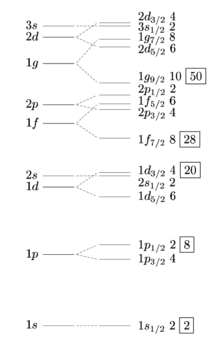
\includegraphics[width=0.45\textwidth]{TeX_files/NuclearShells}
\caption[Nuclear Shell Model level diagram]{From Wikipedia: "Low-lying energy levels in a single-particle shell model with an oscillator potential (with a small negative l2 term) without spin-orbit (left) and with spin-orbit (right) interaction. The number to the right of a level indicates its degeneracy, (2j+1). The boxed integers indicate the magic numbers."}
\label{fig:NuclearShells}
\end{wrapfigure}

Now imagine you stretch out the nucleus somehow. That'll certainly change the spacing and position of the energy levels, because some electron orbitals have a sort of intrinsic shape characteristic that might be better- or worse-suited for the new elongation.

Finally, imagine that you do the stretching \textit{continuously}. That is what is done in a Nilsson diagram. For example, in figure \ref{fig:NilssonDiagram}, the system is elongated from a spherical ground state, and the changing energy levels are the curves, which frequently end up crossing one another. An important thing to notice is that, for different deformations you might have different shell gaps, and as well you might find that different orbitals are more favorable at different deformations.

\begin{figure}
\centering
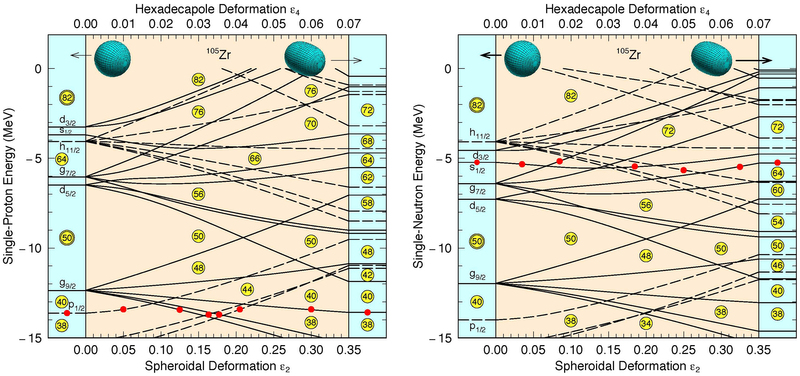
\includegraphics[width=0.7\linewidth]{TeX_files/NilssonDiagram}
\caption[Nilsson Diagram for Zr-105]{Nilsson Diagram for Zr-105, plotted against elongation parameter $\epsilon_2$}
\label{fig:NilssonDiagram}
\end{figure}

Anyway, that's all helpful \textit{once you know} the deformation. And there's a lot of useful and interesting things you can say and predict using a Nilsson diagram - heck, if you know the shape you can [qualitatively] even \textit{draw} a Nilsson diagram, just by thinking about the physical system and how the orbitals are probably behaving.  BUT if you want to understand why a nucleus deforms in the first place, that's a whole other story.

\section{What causes nuclear ground state deformations?}

As with most peculiarities of nuclear structure, the source of nuclear deformation is primarily an artifact of shell structure. In particular, when there is a large shell gap, the nucleus will get sort of "locked" into a particular stable configuration, and if that happens to be a deformed configuration because of the orbital characteristics of the outermost nucleons (because that's the only thing that could matter, right?), then so be it.

A question that I have is how is there ground state deformation in even-even nuclei? Because even-even nuclei all have, without exception, spin-parity $0^+$, and yet $^{152}Dy$ (for example) is highly-deformed. Am I misunderstanding the implications of such a spin-parity assignment? Or am I misunderstanding what is meant by "ground state deformed"?

I don't think this is a real answer, but one way to identify even-even deformed nuclei is to look for nuclei with a large $\frac{E(4^+)}{E(2^+)}$ ratio (or a related method is to look for those with a relatively-small $E(2^+)$).

\section{Phenomenology of Nilsson Diagrams}

[Basically here is where you were thinking about Casten's slides. He goes through and talks about whether a level's energy will go up or down, and how it will curve, just by thinking about the orbital motion of single particles around different axes of the deformed system.]

\section{What causes nuclear ground state deformations? Part 2}
\subsection{What causes fission?}

I think there's a couple of effects at play that lead to fission. First of all, what gets the nucleus moving in the first place, and second, what \textit{keeps} it moving?

To answer the first question, imagine you were to buy a bunch of nucleons at the store and then put them in a box together. Just dump them in with some arbitrary configuration. They'll start to attract and repel one another and there will be kind of a chaotic mess of particle motions to keep track of. TDHF will kind of give you a sense of what's going on in sort of an average sense.

Eventually, the system might settle into a set of sort of normal modes. There will probably be several overlapping normal modes happening at once, so the motion will still look pretty chaotic, but in some average sense you might get something that starts to move with some pseudo-regularity. And with time (I suppose regardless of whether the system motion os regular or not), the system might (for example) elongate, and in fact it might elongate enough for there to be a level crossing in the Nilsson diagram.

When this happens, the system has some deciding to do. It might continue on its current trajectory, or it might jump onto another trajectory (that is, there might be a nucleonic transition from one energy level to another). I suppose it is pretty difficult in practice for a nucleon to make these transitions, because you have all kind of things like conservation of angular momentum and Pauli's principle and such to consider. BUT if you transition a pair of nucleons instead of just one, you can skirt around a lot of these issues, and so I think that's what frequently tends to happen. That is why pairing correlations are sometimes called the "lubricant" of nuclear fission \cite{Bulgac2016}. % Shape deformations
\chapter{Some notes on HFODD}

Since a big chunk of my time has been spent wrestling with the DFT solver HFODD and digging around the source code and whatnot, I thought it would be a good idea to write out at least some of the useful things I've learned that should make it easier for others (or myself) down the line.

First of all, a note on the structure of the code: The actual ``solver,'' or the main function that makes up the skeleton of HFODD only goes to about line 8918 or so in the main file (depending on which version of the code you are using, of course; this figure refers to the Argonne SVN \texttt{branches/inertia} version of the code as of 23 August 2017, for whatever that's worth). A better way to identify it might be to look for the subroutine \texttt{PROANG}, and the main function ends right before that. And actually, the Hartree-Fock iterations don't actually begin until $\sim3820$, and end $\sim8365$; everything before tends to be setup and reading in data and whatnot; everything after is mostly writing data to files.

In fact, it takes a couple hundred more lines of setup inside the loop before any calculations are done, starting with the words ``\texttt{CALCULATING THE MATRIX ELEMENTS OF THE NEUTRON MEAN FIELD}'' and a call to \texttt{INTEGH} (which just adds the individual pieces together, apparently; it doesn't really perform any matrix multiplications). Likewise, it then calculates the neutron pairing field (the matrix elements of the mean-field Skyrme Hamiltonian; multipole constraints are added in there via a call to \texttt{INTCON}). It mixes the HFB matrix, saves the fields, and then diagonalizes the HFB Hamiltonian (\texttt{HFBSI*} in the HO basis, where \texttt{*} depends on symmetries requested by the user). Then it does \texttt{QUABCS}, which calculates the new Fermi energy, followed by a subroutine (for example, \texttt{CANQUA}) which finds and stores the U and V matrices, which transform between canonical and quasiparticle basis. That's another 300 lines. And so what does it do after that? Well, it spends some time computing single-particle average properties (but only when it is ``absolutely necessary''). \textbf{Then} it computes the Skyrme-functional densities and currents (\texttt{DENSHF}), the neutron density matrix, and from there, energies, magnetic moments, the RMS radius, and other properties of the system. That's all done by about line 5000, and then it changes to protons. So it's about 1000 lines of actual HFB calculations for neutrons and about another 1000 for protons (and even less than that, because some of those 1000 lines are just using the computed densities to compute other things). I guess that's not surprising; it's just building and diagonalizing a matrix. Everything else is seeing what cool things you can do with this thing you've just built.

The mean-field matrix diagonalization is completed by $\sim5985$; everything else inside the loop is just bonus physics calculations that take advantage of the newly-computed densities, with some error handling thrown in there as well. So don't be too intimidated by the massive size of the code base; the actual functionality - everything you need to know about the code - is only around 9000 lines (still a lot, but nothing compared to the 200,000 or so lines that make up the entirety of HFODD).

Another thing to note is that there is by default a constraint on $Q_{20}$. There are, of course, plenty of preset values, but this one seems particularly obnoxious. I think there's a way around it but I don't remember off the top of my head what it was. $\rightarrow$ I think you can set the stiffness parameter to zero.

In the table of energies, the so-called ``total energy'' (the very last term in the bottom right) is (so far as I can tell) given by equation I-9 (from the orignal HFODD paper; see also eq VI-96):
\begin{align}
E_{tot} &= E_{kinetic} + E_{Skyrme} + E_{Coulomb} + E_{pair} \\
& + \left[ E_{LN} + E_{pot} + E_{Gog} + E_{Yuk} + E_{CM} + E_{rot} \right]
\end{align}

\section*{Notes on specific subroutines, variables, etc. that I once found useful to know}

Subroutine \texttt{paipri} appears to be printing values it got from the replay file. It uses the variable \texttt{EFER2X} internally, but it is called with \texttt{EFER2N}.

The record file is actually read in ~3447, after some info is printed (\texttt{INFPRI}).

\texttt{ADJBAS} adjusts to find the optimal basis, given the requested value of $Q_{20}$.

\texttt{QMULCM} updates Lagrange multipliers of multipole constraints.

\texttt{QCNTRS} calculates energy contributions due to multipole contraints.

\texttt{INTCON} Calculates multipole moment constraining fields. Called inside \texttt{INTEGH}, which is where matrix elements of the Skyrme mean field are calculated (see eqn 28 of \cite{Dobaczewski1997}). Returns \texttt{HPPCON/HPMCON} (or \texttt{HAUXPP, HAUXPM} as given in the subroutine call).

\texttt{INTEGH} Calculates mean-filed Hamiltonian matrix elements. I believe, but am not positive, that this is eqn 26 in \cite{Dobaczewski1997}. Nothing complicated is really computed in this subroutine; rather, it makes calls to a bunch of subroutines, which individually calculate the different pieces of things found in eqns 27-30, 111, etc, and then just adds the results into a single matrix.

\texttt{DENSHF} Calculates densities (see eqns 40-51 in \cite{Dobaczewski1997}) % Notes on HFODD
\chapter{Nuclear Clusters}

Today I'm trying to read and learn what I can about so-called ``clusters.'' It doesn't sound to me like an inherently difficult concept, but apparently there are some things related to cluster formation that are poorly-understood, and besides that I want to see if I can better improve my study habits by basically keeping a ``study journal.'' So here goes...

My introduction to clustering came from a line in a paper by Nicolas \cite{Schunck2014PES}, where he refers to a small channel in the potential energy surface for $^{240}$Pu corresponding to something called ``cluster radioactivity.''

It comes up quite a bit more with a lot more references in Chunli's first localization paper \cite{Zhang2016localization}. The rest of Chunli's paper doesn't go into much more detail about what clusterization \textit{is}, but it describes a technique for observing shell structure in clusters (or anything, really), even within a ``smeared-out'' DFT framework. It's cool because DFT tends to blur and spread out the impact of single-particle wavefunctions across the entire nuclear volume, but this localization technique gives you a way to see something shell-like within the nucleus. That's especially useful in fission because the formation of fragments is driven by the shell structure of the pre-fragments (and not the final fragments themselves). So if you start to see shell structure appearing in your scissioning nucleus, you might be able to say something about what the final fragments are, just based on the shell structure of the pre-fragments.

But I'm still skeptical. $^{86}$Kr and $^{84}$Se will probably have almost identical shell structure (magic $N=50$ for neutrons, and an off-shell even number of protons). Is it really likely that you'd be able to identify the different isotopes just using the localization measure? I actually tested something very much like this back for platinum-176. There I actually used an even more extreme example of $^{84}$Se, $^{82}$Se, and $^{86}$Zr. The seleniums were almost identical (the neutron spatial localization was only very slightly different), and the zirconium was even \textit{pretty} similar (whatever that means). You can see the results somewhere on my computer where I have them stored, and I also showed a few sample figures in the \texttt{research\_notes.tex} file, under \textbf{Nucleon Localization Function \rightarrow 28 September 2017}

But I digress...

Apparently historically, the idea of cluster emission was originally characterized by situations where the emitted fragment was larger than an alpha particle, but capped off at about $Z_e^{max}=28$ (see the introduction to \cite{Warda2011} for kind of a historical overview of cluster radiation). However, starting in around 2012 and taking into account results from heavy and superheavy systems, the criteria was relaxed to allow for $Z_e>28$. They had noticed that very often the larger remaining fragment was $^{208}$Pb or one of its neighbors, and so now cluster emission includes heavy fragments up to $Z_e^{max}=Z-82$ (see \cite{Poenaru2012}). Physically, it's basically the same thing happening (lead sheds whatever is left and the rest forms a cluster); the only major difference is that superheavy isotopes can produce heavier clusters. Several models have been proposed to describe the phenomenon, such as superasymmetric fission or tunneling of a preformed fragment through a potential barrier. We actually have a bit of useful information we can use to test that. If you look in my \texttt{research\_notes.tex} file, under \textbf{Nucleon Localization Function \rightarrow 29 September 2017} you can see some nice diagrams that show the development of shell structure in the fragments of $^{294}$Og. Based solely on this set of results, I don't feel comfortable with the idea of a preformed fragment tunneling through a potential barrier - at least not for the smaller fragment. Look at the proton localization for krypton and you'll see that its shell structure doesn't develop until fairly late. The lead develops fairly quickly, however, and I believe that was the conclusion reached in \cite{Warda2011}.

Michal Warda gave a[n unpublished] presentation in September 2017 about cluster radioactivity in superheavy nuclei. He showed some cool pictures of potential energy surfaces evolving from actinides to superheavies, and you can totally see cluster emission go from a very unlikely branch to perhaps the dominant fission channel. Ultimately his conclusions are:

\begin{itemize}
\item Asymmetric fission in superheavy nuclei region has the same nature as cluster radioactivity in actinides
\item This decay may be dominant in some superheavy nuclei
\item Sharp fragment mass distribution with $^{208}$Pb fragment is predicted
\end{itemize}

Cluster formation in actinides generally seems to be associated with a fairly long half-life (typically $10^{11}-10^{26}$ seconds, according to Warda's presentation; see also \cite{Poenaru2011} and references therein) and a low branching ratio relative to $\alpha$ decay ($10^{-9}-10^{-16}$). However, he also shows a drastic reduction in the size of the barrier to cluster formation, from upwards of 25 MeV down to around 5 MeV, and I suspect the half-lives will see a major reduction as a consequence. It's impossible to say for sure without actually \textit{doing} the calculation, but I suspect just from looking at the barrier that it'll be comparable with asymmetric fission in actinides or shorter. Figure 4 in \cite{Poenaru2011} makes it look like $\alpha$ decay will win out over cluster radioacitivity only \textit{just barely}, with a half-life only perhaps a factor of 10 shorter.

Also worth noting is that ``Several attempts to detect $^{12}$C radioactivity of the neutron deficient $^{114}$Ba
with a daughter in the neighborhood of the double magic $^{100}$Sn, predicted to have a larger $b_\alpha$, have failed'' \cite{Poenaru2011}. So it seems to be a phenomenon linked to lead or, more likely, heavy and superheavy elements. Seeing that for superheavy elements, cluster emission and asymmetric fission appear to be one and the same, it makes sense to think of cluster emission as a particularly asymmetric instance of regular, garden-variety fission.

\subsection*{A note about ``clusters''}
The notion of a ``cluster'' is not, so far as I can tell, rigorously-defined. In all I've said leading up to this, cluster radiation/cluster emission is the process by which lead (or some lead-like nucleus) sheds its excess nucleons, and whatever is left just forms into its own so-called ``cluster.'' So in that case, a cluster is just a clump of leftover nucleons.

But as I say, that is not totally rigorous. Bastian and Witek published a paper (I should say, they \textit{submitted} a paper, because at the time I am writing this, it is only available on the arXiv: https://arxiv.org/abs/1710.00579) where they discussed ``cluster formation in pre-compound nuclei.'' Their argument was that entrance channel effects can't necessarily be ignored in various collisions involving compound nuclei, because sometimes the nucleus isn't as thermalized as we'd like to think (we haven't lost all the information about the incoming particles). $\alpha$ particles in particular like to stick together and move around in clumps. So in that case, ``clusters'' refers to substructures within the overall system (like $\alpha$ particles hanging out at the tips of an elongated nucleus, or rings of carbon-12 forming near the middle).

There's probably no real need to overthink this: ``cluster'' is just a useful word that describes organized nuclear structures which are smaller than the overall system under consideration. I don't think anyone means anything more than that. Or at least, they probably shouldn't.

\subsection*{Alpha Clustering}
An interesting question that hasn't been immediately obvious to me is how to deal with the concept of alpha clusters. I don't see a channel on my PES corresponding to an alpha decay. Perhaps it might manifest itself as a very narrow, deep channel that doesn't show up with the resolution of my current oganesson surface. So I wanted to see what else people had come up with to predict alpha decay half-lives, and especially to see if there was anything more than just phenomenological hand waving. And it turns out the answer is yes. From what I understand, alpha decay (at least according to this thesis and the papers cited therein: http://uir.unisa.ac.za/bitstream/handle/10500/1220/dissertation.pdf) involves $p-p$ and $n-n$ pairs forming in high-lying states near the surface, with $p-n$ pairing giving the final catalyst to let a particle shed off (configuration mixing).

\subsection*{Remaining questions}
Since localizations can be used to visualize clusters, I'm going to posit a question here (which was originally suggested by Gregory Potel): Would it be possible to visualize pairs, and not just individual nucleons? If so, it might be interesting to see how pairs move around as you near scission (perhaps especially as part of a time-dependent calculation). % Nuclear clustering
\chapter{Bayesian Inference}

A lot of my notes on statistical inference are in my UQ class notes from Fall 2017 with Mohsen Z, but I have some more fundamental questions that I'd like to understand and I think writing down insights as they come will ultimately prove helpful.

\section{Bayes' Theorem}

Let's say you have a model of some system, but you don't know the coefficients or parameters of the model. But you do have a bunch of data, and you'd like to use that data to go back and figure out what the model parameters probably are. For instance, in a coin toss, you might have a model like $H(f) = \alpha*f$, where $f$ is the number of flips and $H$ is the number of heads. You've done the experiment a hundred million times and you want to use your data to come up with some estimate for the coefficient $\alpha$ (and perhaps even an uncertainty). You might also have some inkling of what that coefficient should be - for sure you know that it will be somewhere between 0 and 1, but maybe you have reason to believe that it's even somewhere in the interval [0.37, 0.54], or that coin-flipping coefficients are manufactured around a normal distribution centered about 0.53.

The essence of Bayes' Theorem says that if you fold together everything that you know (your data) with what you suspect (your ``prior''), then you can update your suspicion (your ``posterior,'' which can in turn become a prior in your next round of estimation) to give you something probably better. Depending on the ``forcefulness'' of your prior, or the amount of data you've collected, you might see that the data completely overwhelms the prior, or vice versa.

The prior could be anything from a flat line (if you have no idea what to expect) to a delta function (though I wouldn't recommend using that since it makes your posterior also a delta function unless you know for a fact what to expect, but then why are you even doing this?).

The likelihood is where you work your data in. An example likelihood function might involve an exponential of a chi-squared function, for example ($P(D|H) \sim exp(-\frac{\chi^2}{2})$). This would give some sort of distribution that is peaked at the ``best fit'' set of parameters. In general, a likelihood tells you ``How likely was this outcome, given these parameters?'' whereas the posterior tells you ``How likely are these parameters, given the outcome?''

[These StackExchange questions has some helpful discussion: \\ https://stats.stackexchange.com/questions/58564/help-me-understand-bayesian-prior-and-posterior-distributions \\
https://stats.stackexchange.com/questions/2641/what-is-the-difference-between-likelihood-and-probability]

\section{Markov Chain Monte Carlo}

Let's say we have a set of data $D$ and a model hypothesis with parameters $H$. Then Bayes' Theorem in this case might look like:

\begin{equation}
P(H|D) = \frac{P(D)P(D|H)}{P(H)}
\end{equation}

Just for the sake of argument, our prior and likelihood might take the following forms:

\begin{align}
P(D) &\sim exp[\frac{1}{2}(\vec{x}-\vec{x}_0)^TC_p^{-1}(\vec{x}-\vec{x}_0)] \nonumber\\
P(D|H) &\sim exp[\frac{\chi^2}{2}] \nonumber\\
\chi^2 &= \sum_i\left[\frac{\sigma^{th}(\vec{x})-\sigma^{exp}}{\Delta\sigma}\right]^2 \nonumber
\end{align}

\noindent Maybe we want to estimate the sample distribution for the parameter $x_1$. We could do that essentially by integrating the posterior over all other parameters:

\begin{equation}
P(H_1|D) = \int P(D)P(D|H)dx_2dx_3\dots dx_n
\end{equation}

In principle, this makes sense. You get a nice-looking one-dimensional distribution of values of $x_1$ as sort of a histogram. In practice, though, that integral is probably really hard to solve. So instead you can turn to a method called Markov Chain Monte Carlo. In there, you pick a starting point in your sample space, and then you just do sort of a random walk (described by your Markov Chain). You take a bunch of steps, and you keep the ones that satisfy a set of conditions \footnote{You'll probably evaluate the prior and likelihoods at the old step and the new step, compute their ratio, and only keep the point if the ratio $\frac{\mathnormal{new point}}{\mathnormal{old point}}>1$}. From these saved/logged/archived steps, you can put together essentially a histogram that represents the posterior distribution for that parameter.

``But Zachary!'' you might ask. ``If you're only keeping points that give an improved ratio, then won't you converge quickly to the 'true' value, and not have much to show in the tails?'' And the answer is ``not necessarily.'' It might be that your prior is way out in the tails, for instance, and so your random walk might heavily favor those values at first until you have enough data to override. Or perhaps you're in a weird saddle/local minimum of your multidimensional space where improving one parameter requires you to reduce the quality of another. Or perhaps you have a complicated, ill-posed, non-linear model where converging to the ``true'' parameter (which doesn't really even exist in Bayesian statistics, but let's pretend) might not immediately converge to the true value ($\lim_{x\rightarrow x_{true}}\sigma^{th}(x) \neq \sigma^{exp}$ over some range of $x$). % Bayesian Inference
\chapter{UQ for Nuclear DFT}

\section{Introduction}
A recent goal in nuclear physics has been to develop models with quantified uncertainties (I wonder - where did that push start? Was it within the theory community? A request from experimentalists? A mandate from the funding sources?). One of these models - DFT - is useful all across the nuclear landscape. A recent collaboration sought to develop a UNiversal Energy Density Functional - hence the name of the collaboration, UNEDF. This family of three energy density functionals was designed to be applied across the entire nuclear chart, and each member of the set had a particular focus in mind: UNEDF0 was a proof of concept, UNEDF1 was optimized for large nuclear deformations, and UNEDF2 is designed to effectively capture the physics of shell structure. Furthermore, these functionals were designed with UQ in mind; each functional has an evaluated covariance matrix, and sensitivity analyses were performed for each of the parameters.

\section{Compiling a list of uncertainties}
So far I'm just brainstorming by outlining essentially every possible source of error or uncertainty I can think of in the physical model and its numerical implementation. At each step I'll discuss both some short- and long-term suggestions for ways to improve the outcome.

\subsection{Nuclear Force}
\begin{itemize}
\item We don't really \textit{know} the nuclear force, per se... (my understanding is that it's just a residual interaction from the QCD interaction of the constituent quarks)
\item Skyrme, Gogny, etc
\item EDF parameterization
\item EDF fitting strategy
\item Coulomb\dots
\item The mean-field approximation, and consequently, the pairing interaction - or in other words, correlations that go beyond just the mean-field
\item \dots
\end{itemize}

\subsection{DFT Solver}
I should mention here that there is some brief discussion at the beginning of the very first HFODD paper about different numerical techniques that can be (and perhaps \textit{have been}) used to solve the HF(B) equations, such as finite-difference or conjugate gradient methods (see also subsection 7.3.3 of Ring and Schuck).

\begin{itemize}
\item Basis size - number of states, shells
\item Basis type
\item Integration mesh
\item Determining convergence - That's hard to quantify exactly; it may be that we converge to a local, but not global minimum.
\item Calculation of $V_{eff}$ (subtracting off zero-point energy?)
\item The whole thing about using a ground state-based method to calculate highly-deformed nuclei
\item \dots
\end{itemize}

\subsection{Inertia}
\begin{itemize}
\item Recipe for calculating (perturbative vs. nonperturbative, ATDHF vs GCM)
\item Adiabatic approximation - ``slow'' collective motion
\item Finite difference spacing
\item Cutoff parameter (for finite temperature)
\end{itemize}

Here there's a divergence which determines what comes next

\subsection{Half-life, Pathway to Fragments}
\begin{itemize}
\item Validity of WKB approximation
\item Semi-classical SF half-life approximation
\item Parameters determining frequency of tunneling attempts
\item Interpolation of potential energy surface
\item Choice of collective coordinates
\item Choice of $E_0$ 
\item Identification of scission line
\item Identification of least-action path inside the barrier (Dynamic programming method vs. Ritz method [vs. static least-energy path])
\item Effectiveness of Langevin description of dynamics outside the barrier
\item \dots
\end{itemize}

\section{Review of the DFT error analysis survey article \cite{Schunck2015}}

There are two schools of thought when it comes to DFT, apparently. One is ... I'm not totally sure what the distinction is, actually. The first has something to do with building a self-consistent mean-field (and my impression is that's done \textit{from scratch}, in some sense.) The other (which is what I'm familiar with) starts with a rather phenomenological potential (perhaps a Skyrme interaction), as opposed to one built from the ground up. Then you somehow come up with a set of parameters to tweak that Skyrme interaction. That's where the UNEDF project takes off.

Essentially what this paper tries to do in the end, though, is to discuss the three types of uncertainties that can affect your DFT calculation results. There are numerical errors, which are pretty easy to understand and likewise to quantify. For example, in an iterative scheme, you can increase the number of iterations and see how the convergence of your solution is affected. Or if your calculation depends on a basis expansion, you can try running the calculation with different basis sizes and seeing what happens. As a general rule of thumb, if you want to quantify numerical errors, it's probably just a matter of increasing the number of iterations/increasing the size of the basis/using a finer mesh. Nothing too mysterious here.

Harder to quantify is the effect of your theoretical model itself. Intuitively we believe that a DFT calculation should give better results than a liquid drop model calculation, or ab initio potentials will be superior to phenomenology, but it doesn't always work out that way and oftentimes (if you're extrapolating your model) it's impossible to quantify. We assume that our description of the nucleus will be incomplete whenever we use a Skyrme-based potential, but we don't really know \textit{how} incomplete. And it's not obvious how to go about determining that, short of just comparing against experiment (but again, you really have to be able to tease out your numerical error and your fitting bias). That's why it would be nice to have either potentials, or at least coupling constants derived somehow from theory, and not just fit to data. Because if you can fit your coupling constants from theory, then at least you know what approximations it took to get from ``exact'' to ``approximate.'' So a good question to answer would be ``How could we get from the basic NN-interaction to Skyrme?'' Is such a thing even possible? Skyrme is phenomenological, but maybe it could emerge from an analytic NN interaction somehow? If only we had an analytic form for a NN interaction (or even approximation that was analytic)...

But wait - isn't that what Skyrme \textit{is}? Oh gosh, we're hosed...

Anyway, the other thing to quantify here is the uncertainty in your model parameters. These are separate from the shortcomings of the model itself - you accept that your model is off by some amount, because of what you might consider a systematic error in your model (a missing bit of physics, for instance). Already you can see how hard it is to tease apart your model uncertainty and your model parameter uncertainty, because what we're about to ask you to do is to find the exact parameters to an inexact model. What would that even mean? So maybe you settle for a ``best'' set of parameters. Okay, fine. Still tough to do ``exactly.'' For one thing, your fit will depend on the numerical implementation of the model (all that stuff about basis size, number of iterations, grid spacing, etc again applies, plus maybe some assumptions made in the solver that restrict it to a certain subset of the full model). Then it also depends on the optimization scheme you use (least squares fitting or something else). And finally, it depends on the experimental data you feed into it. In fact, there have been a few studies aimed at understanding the impact of different types of data on your final results (a few are mentioned towards the end of section 4.1, and there is also the paper done my Jordan, Nicolas, Witek, and others \cite{McDonnell2015}).

These points are supplemented with some examples from the UNEDF project, showing how difficult it can be to tease apart the different sources of uncertainty but trying anyway. They talk a bit about the Bayesian problem they solved to do the fitting, and then about some of the assumptions they made in order to compute the covariance matrix and such, and tried to argue whether those assumptions were reasonable or not. To really understand what was done beyond these illustrative introductions, though, I imagine I'll need to look back at the original papers. So next stop: UNEDF0!

\section{Review of the UNEDF0 paper \cite{Kortelainen2008}}

Something cool about this, right off the bat after reading the abstract, is that they gained ``new physics insights...by the advanced covariance analysis.''

There's a nice brief review of some of the other parameter-fitting schemes that have been attempted. Those are nice because they help to understand better the nature of parameter-fitting uncertainties.

In practice, the way things worked was to take their DFT solver and compile or run it inside a wrapper code (\texttt{POUNDERS}, I believe) that took care of the statistics part, and called on the DFT solver whenever it needed something.

The first thing they did was they tried to find, for as many parameters as possible, a sensible range of values in which to do a parameter search. The EDF terms are not directly-related to any observable quantities; however, the equation of state for infinite nuclear matter can be recast both in terms of observable quantities as well as Skyrme functional densities and coupling constants, and from there we can draw an approximate relation between the two. Then, since we have a rough idea of what the equation of state physical quantities of interest/scale are, we have a good starting place for our parameter search.

Then a set of experimental data was chosen to represent the chart of nuclides as a whole. This set has been published as a standard set of data for model calibrations, to reduce the uncertainty related with choice of experimental data.

\section{Review of ``Error Estimates of Theoretical Models: a Guide'' \cite{Dobaczewski2014}}


\section{Miscellaneous}

This paper (https://e-reports-ext.llnl.gov/pdf/790483.pdf) has a nice table (Table 2) which shows the impact that your input starting points have on your final solution, even using the same algorithm and the same data points. That's very interesting, actually, because in most cases, the difference between starting and ending points have the same sign, and the starting and ending points almost have the same rough magnitudes between functionals.

This paper (J. Phys. G: Nucl. Part. Phys. 42 (2015) 034031) does more-or-less the same thing.

I don't have a section on chiral EFT, but an essential idea from that, which I learned from a Dick Furnstahl talk, is that if you can identify a scale in your expansion, then in nice systems (like relativity or presumably chiral EFT), your coefficients will be of roughly the same order, which means you can estimate truncation errors with some confidence.
 % UQ for Nuclear DFT
\chapter{HFB, DFT, and Beyond Mean-Field Corrections}

\maketitle

Beyond mean-field corrections are used to include correlations which are discarded or distorted through the HFB/SCMF formalism. Some of these may deal with configuration mixing and collective motion, and these are treated using the Generator Coordinate Method. Other corrections are used to impose symmetries which are found in nature but which are violated in the mean-field calculation. I am going to explain these latter beyond mean-field correction in the context of Lipkin-Nogami, which is used to compensate for the loss of particle-number conservation due to the Bogoliubov transformation. There are, as I will mention later, other such corrections one can make, such as a rotational correction to restore good angular momentum, for instance. For more, one can read p.15 of Nicolas Schunck's and Luis Robledo's review article on fission \cite{Schunck2016review}, or especially section III-B of Michael Bender, et al's review article on self-consistent mean-field models \cite{Bender2003}.

\section*{Lipkin-Nogami}
The Lipkin-Nogami method of restoring particle number symmetry to the nucleus involves splitting the energy density into two terms:
\begin{equation*}
\mathcal{E}_{TOT} = \mathcal{E}_{HFB} + \mathcal{E}_{LN}
\end{equation*}

\noindent where $\mathcal{E}$ is computed as

\begin{equation*}
\mathcal{E}_{LN} = -\lambda_2\left(\left\langle N^2\right\rangle -N^2\right) = -2\lambda_2 \mathrm{Tr}\rho\left(1-\rho\right)
\end{equation*}

Lipkin-Nogami is an example of a beyond mean-field correction. Beyond mean field corrections are used to restore symmetries which are otherwise broken in the HFB equations, such as particle number conservation, a good angular momentum number (rotational invariance correction), or parity. Once the HFB solution is obtained, the conserved quantity is restored (in principle) by projecting your solution back onto the space of solutions with good quantum numbers. In principle, this projection should be done before variation (VAP), so that the wavefunctions from which the variational principle draws are only those which have the correct symmetries. However, VAP methods are quite challenging. You can approximate the effect by swapping the order (PAV). Here you take whatever solution successfully minimizes the HFB equations and then project \textit{that} onto the space of ``good'' wavefunctions. It's easier sometimes than VAP and may get you close, but of course it is not guaranteed that you'll get the correct answer.

Sometimes even pure PAV is too hard, and you might want a simpler, more ``phenomenological'' way of guessing the effect of VAP. You do your mean-field HFB calculation, get some answer $|\Psi\rangle$, and then use some formula to estimate what the effect of VAP \textit{would have} been on your variational energy, had you done it that way. This is what Lipkin-Nogami is for particle number restoration. You solve the HFB equations at the mean field level, and instead of properly projecting your states onto states with good particle number symmetry, you calculate a correction term to your energy to estimate the effect that proper projection would have had. You can calculate the particle number variance $\langle\Delta \hat{N}^2\rangle$ just from your densities, and there is a recipe for calculating $\lambda_2$ from your density as well (see eqn 92 of Bender, et al, Rev Mod Phys 75 (2003), or see how it is implemented in HFODD below). In this case, since you are not actually using Lipkin-Nogami to do particle number restoration (even approximately), then the Lipkin correction term to the energy is not physical. The number you want, and which you actually have available, is the original mean-field solution \textit{without} any beyond mean-field corrections (or, I mean, you can add other ones, but just know that the ``default'' energy HFODD is giving you is including a Lipkin energy which is not a correct beyond mean-field correction to the energy).

Worth mentioning is the fact that, at least in HFODD, the Lipkin-Nogami term is included as part of the variational energy. So you aren't minimizing with respect to the pure HFB energy, but rather the pure HFB energy PLUS the Lipkin-Nogami correction term. Hopefully you appreciate this distinction, and understand that it can have an effect on the overall properties of your system.

In your 4D oganesson calculation (and in Jhilam's paper about pairing correlations in fission), you do something just a little bit different. You aren't doing Lipkin-Nogami, but you do something similar, but for a completely different purpose. Here you fix the value of $\lambda_2$. By doing so, you effectively impose that particle number variance will have a certain ``importance'' to the system: higher $\lambda_2$ means that particle number fluctuations are more important to your system than if you had a smaller $\lambda_2$. Since this correction term to your energy is included in the variation, then you are baking this preference into your solution. And since large particle number fluctuations are tied to stronger pairing, then by imposing a large value of $\lambda_2$ you are indirectly imposing a large pairing strength ($V_0$) into your system (and this in turn manifests itself through a larger pairing gap $\Delta$ and a larger pairing energy).

In HFODD, $\lambda_2$ is evaluated on every iteration using the updated densities form the previous iteration, starting from some initial value you can set in the input. It is also possible in HFODD to fix the value of lambda and not update it for each new iteration, if you're into that kind of thing. It is given approximately via the seniority-pairing interaction by

\begin{equation*}
\lambda_2 = \frac{G}{4}\frac{\mathrm{Tr}(1-\rho)\kappa \mathrm{Tr}\rho\kappa-2\mathrm{Tr}(1-\rho)^2\rho^2}{\left[\mathrm{Tr}\rho(1-\rho)\right]^2-2\mathrm{Tr}\rho^2(1-\rho)^2}
\end{equation*}

\noindent where

\begin{equation*}
G = G_{eff} = -\frac{\bar{\Delta}^2}{E_{pair}}, \qquad E_{pair} = -\frac{1}{2}\mathrm{Tr}\Delta\kappa, \qquad \bar{\Delta} = \frac{\mathrm{Tr}\Delta\rho}{\mathrm{Tr}\rho}
\end{equation*}

The UNEDF functionals included pairing strengths for both protons and neutrons as part of the Skyrme parameter set when they were optimizing, so the pairing strength is actually given as a parameter instead of computed from the densities in (for example) HFODD $\leftarrow$ Double-check this! But I think that's how it'll work? I'm getting lost in the source trying to find out... (4-19-2017) But definitely you shouldn't use Lipkin-Nogami with the EDF UNEDF1-HFB. That was explicitly computed \textit{without} Lipkin-Nogami. You could set the lambdas all you want but they won't do a darn thing, unless you turn on Lipkin-Nogami but that'd be dumb because then you'd get the wrong answer.

\section*{Unresolved questions}
Aside from not really knowing how GCM or GOA work, I also don't quite understand why it is that symmetry-restoring corrections apparently tend to lower the total energy. The way I'm seeing it now is (at least for PAV): you have a solution which minimizes your HFB energy, and it is some linear combination of wavefunctions which may or may not have the correct symmetries. So you project out the ones that aren't helping and only keep the ones with good quantum numbers. And somehow this should lower your overall energy? I mean, unless you're like averaging the energy over wavefunctions, and somehow the wavefunctions with good quantum numbers have the lowest energy. Then by cutting out the others you'd allow your average to settle into that lowest value. And in reality, I suspect the truth is something like that - maybe not averaging, of course, but it might make sense that the states with good quantum numbers are optimized for the Hamiltonian density you started with, which has a symmetry-restoring-on-the-average term. So I dunno. Am I barking up the wrong tree?

\section*{Functionals for odd-mass nuclei}
This is admittedly not a beyond-mean field concept, but it is in some sense beyond the standard mean field calculations I'm used to.

There are I suppose four ways to fit a functional to odd-mass nuclei/time-odd terms:
\begin{itemize}
	\item Derive the functional from a force (Skyrme, for instance. This is more in line with SkM* than UNEDF)
	\item Impose local gauge invariance
	\item Landau parameters (See Osterfield 1992, with a 2018 PRL involving Remco Zegers for an update)
	\item Ignore the time-odd terms altogether.
\end{itemize}

These ideas are discussed in PRC 81 024316 by Schunck et al (https://doi.org/10.1103/PhysRevC.81.024316).

\section*{Single-reference vs. multi-reference HFB}
Another not-necessarily beyond-mean-field concept that I'm going to discuss here is the notion of single-reference vs multi-reference HFB. What you're used to is single-reference, and so far as I can tell that name comes about because you calculate everything with respect to a single Slater determinant - the vacuum state. GCM is a multi-reference extension of what you're familiar with. The foundation of GCM is that you construct a wavefunction that is a coherent superposition of different HFB states, as opposed to just a single one.

There is an analog within EDF theory - MR-EDF vs SR-EDF. Essentially there you're just dealing with density matrices instead of wavefunctions, but you already know how that goes.

See \verb|http://www.int.washington.edu/talks/WorkShops/int_13_1a/People/Bender_M/Bender.pdf|

\section*{Convergence of HF/HFB iterations}
A question I've wondered about is how do we have any kind of assurance that our HFB iterations will even converge? Like, we diagonalize the matrix and use the result to construct a whole new problem. Who's to say that the solution to this entirely-new problem will be anywhere even close to the original problem/solution? And it turns out that is exactly true. I mean, you've already had plenty of cases where a bad initial guess led to a chaotically diverging result (or some other kind of divergence), so you're already aware that convergence isn't guaranteed. But I wanted to know more! And it turns out, so did someone else on the internet. Here's a stackexchange post about exactly this: https://scicomp.stackexchange.com/questions/1297/why-does-iteratively-solving-the-hartree-fock-equations-result-in-convergence

Not only do they answer the question (``No, convergence isn't guaranteed''), but they also manage to provide some conditions under which convergence \textit{is} guaranteed, and furthermore they give some algorithms and tools that help encourage convergence. In case the link ever breaks, here are the two best answers:

Answer \#1
\begin{quote}
The Hartree-Fock equations are the result of performing constrained Newton-Raphson minimization of the energy with respect to the parameter space of Slater determinants (I don't have my copy of Szabo-Ostlund at hand, but I believe this is pointed out in the derivation). Hence, HF-SCF will converge if your starting guess is in a convex region around a minimum. Elsewhere, it may or may not converge. SCF convergence fails all the time.
answered Feb 13 '12 at 12:54
Deathbreath

The impression I am getting is that the SCF method only converges if (i) the function is well behaved and (ii) the initial guess occurs sufficiently near the global minimum. Would you agree with this? – James Womack Feb 14 '12 at 11:28

It need not be near the global minimum. For instance, you might be trapped in a symmetry with a local minimum that isn't global. If the function is ill-behaved, I agree that you will most likely not converge. I encourage you to derive the gradient and the Hessian of the HF energy functional w.r.t. the orbital coefficients yourself and compare them to the Fock matrix. Nocedal's book on optimization is great for understanding the convergence behavior in this light then. – Deathbreath Feb 14 '12 at 13:01

Even if you're near a minimum, you can still have problems with systems that have closely spaced minima or low-curvature potential surfaces. In particular in my experience, systems like actinide (and I assume lanthanide) compounds with near-degenerate levels and states around the minimum tend to be difficult, since your optimiser can repeatedly overshoot the actual minimum. (Which is where damping comes in handy.) – Aesin Feb 14 '12 at 20:15
\end{quote}

Answer \#2
\begin{quote}
	Density functional theory (DFT) also uses a one-particle approach similar to Hartree-Fock, although the effective potential is a little more involved. To achieve a global minimum, the problem is approached as a non-linear fixed point problem which, as Deathbreath said, can be solved via a constrained Newton-Raphson minimization. A common approach in the DFT community is to use Broyden's Method which if organized correctly (J Phys A 17 (1984) L317) requires only two vectors: the current input and output. (See Singh and Nordstrom, p. 91-92, for a quick overview of this method, or Martin, Appendix L, for a more complete overview of related techniques.) A more recent technique used in Wien2k attempts to overcome convergence difficulties with the Broyden method by employing a multi-secant method.(PRB 78 (2008) 075114, arXiv:0801.3098)
	answered Feb 13 '12 at 16:55
	rcollyer

	Another approach other than using quasi-Newton methods (Broyden) would also be DIIS. – Deathbreath Feb 13 '12 at 18:38
\end{quote} % Beyond mean-field corrections to the energy

\backmatter
% bibliography, glossary and index would go here.
\bibliography{main}
\bibliographystyle{abbrv}

\end{document}